\documentclass[11pt, letterpaper]{article}

% Fonts and Encoding
\usepackage[utf8]{inputenc}
\usepackage[T1]{fontenc}
\usepackage{lmodern} % High-quality Latin Modern vector font

% Math and Symbols
\usepackage{amsmath, amssymb, amsthm, amsfonts, mathrsfs, mathtools}

% Layout and Geometry
\usepackage{geometry}
\geometry{letterpaper, margin=1in}
\setlength{\parindent}{0pt}
\setlength{\parskip}{0.6em}

% Formatting and Graphics
\usepackage{graphicx, xcolor, enumitem, booktabs, array, tabularx}

% TikZ for Illustrations
\usepackage{tikz}
\usetikzlibrary{arrows.meta, positioning, shapes.geometric, calc, backgrounds, matrix}

% Clickable Links and TOC
\usepackage{hyperref}
\hypersetup{
    colorlinks=true,
    linkcolor=blue,
    filecolor=magenta,      
    urlcolor=cyan,
    pdftitle={Advanced Mathematics Topic},
}

% Theorem Environments
\newtheorem{theorem}{Theorem}[section]
\newtheorem{lemma}[theorem]{Lemma}
\newtheorem{proposition}[theorem]{Proposition}
\newtheorem{corollary}[theorem]{Corollary}
\theoremstyle{definition}
\newtheorem{definition}{Definition}[section]
\newtheorem{axiom}{Axiom}[section]
\newtheorem{example}{Example}[section]
\theoremstyle{remark}
\newtheorem{remark}{Remark}[section]

% Custom Commands (Enforced standard notation)
\newcommand{\R}{\mathbb{R}}
\newcommand{\N}{\mathbb{N}}
\newcommand{\Z}{\mathbb{Z}}
\newcommand{\Q}{\mathbb{Q}}
\newcommand{\E}{\mathbb{E}}
\newcommand{\Prob}{\mathbb{P}}
\newcommand{\F}{\mathcal{F}}

\title{\textbf{The Method of Distribution Functions: Measure-Theoretic Foundations, Pushforward Measures, and Quantitative Applications}}
\author{Tashfeen Omran}
\date{\today}

\begin{document}

\maketitle
\tableofcontents
\newpage

% ============================================================================
% PART 1: COMPREHENSIVE INTRODUCTION, CONTEXT, AND PREREQUISITES
% ============================================================================
\section{Comprehensive Introduction, Context, and Prerequisites}

\subsection{Core Concepts and Axioms}

In elementary calculus-based probability, finding the probability distribution of a function of random variables $U = h(Y_1, Y_2, \dots, Y_n)$ is often treated as an exercise in changing limits of integration. However, in advanced abstract mathematics and modern probability theory, **The Method of Distribution Functions** is the concrete analytical manifestation of the **pushforward measure** (or image measure) induced by a measurable mapping between measurable spaces, coupled with the **Radon-Nikodym Theorem** and the **Fundamental Theorem of Calculus for Lebesgue Integrals**.

To establish this theory from the ground up, we first define the underlying mathematical structures.

\begin{definition}[Measurable Space and Probability Space]
A \textbf{probability space} is a measure-theoretic triple $(\Omega, \F, \Prob)$, where:
\begin{enumerate}[label=(\roman*)]
    \item $\Omega$ is a non-empty set called the \textbf{sample space}, whose elements $\omega \in \Omega$ represent elementary outcomes.
    \item $\F \subseteq \mathcal{P}(\Omega)$ is a \textbf{$\sigma$-algebra} (or $\sigma$-field) of subsets of $\Omega$, meaning:
    \begin{enumerate}[label=(\alph*)]
        \item $\Omega \in \F$;
        \item If $A \in \F$, then $A^c = \Omega \setminus A \in \F$ (closure under complementation);
        \item If $\{A_k\}_{k=1}^{\infty} \subset \F$, then $\bigcup_{k=1}^{\infty} A_k \in \F$ (closure under countable unions).
    \end{enumerate}
    \item $\Prob : \F \to [0, 1]$ is a \textbf{probability measure} satisfying the **Kolmogorov Axioms**:
    \begin{enumerate}[label=(\alph*)]
        \item \textit{Non-negativity:} $\Prob(A) \ge 0$ for all $A \in \F$.
        \item \textit{Normalization:} $\Prob(\Omega) = 1$.
        \item \textit{Countable Additivity ($\sigma$-additivity):} For any countable sequence of pairwise disjoint events $\{A_k\}_{k=1}^{\infty} \subset \F$ (where $A_i \cap A_j = \emptyset$ for $i \neq j$),
        \[
            \Prob\left(\bigcup_{k=1}^{\infty} A_k\right) = \sum_{k=1}^{\infty} \Prob(A_k).
        \]
    \end{enumerate}
\end{enumerate}
\end{definition}

\begin{definition}[Random Vector and Pushforward Law]
Let $(\Omega, \F, \Prob)$ be a probability space, and let $(\R^n, \mathcal{B}(\R^n))$ be the $n$-dimensional Euclidean space equipped with its **Borel $\sigma$-algebra** $\mathcal{B}(\R^n)$ (the smallest $\sigma$-algebra containing all open subsets of $\R^n$). A function $\mathbf{Y} = (Y_1, Y_2, \dots, Y_n) : \Omega \to \R^n$ is a \textbf{random vector} if it is $(\F, \mathcal{B}(\R^n))$-measurable, meaning that for every Borel set $B \in \mathcal{B}(\R^n)$, the preimage
\[
    \mathbf{Y}^{-1}(B) = \{\omega \in \Omega : \mathbf{Y}(\omega) \in B\} \in \F.
\]
The random vector $\mathbf{Y}$ induces a **pushforward probability measure** (or **law**) $\Prob_{\mathbf{Y}} : \mathcal{B}(\R^n) \to [0,1]$ defined by
\[
    \Prob_{\mathbf{Y}}(B) \coloneqq \Prob\left(\mathbf{Y}^{-1}(B)\right) = \Prob(\mathbf{Y} \in B).
\]
\end{definition}

\begin{definition}[Cumulative Distribution Function and Absolute Continuity]
Let $U : \Omega \to \R$ be a real-valued random variable. Its **Cumulative Distribution Function (CDF)** $F_U : \R \to [0, 1]$ is defined for all $u \in \R$ by the measure of the semi-infinite Borel interval $(-\infty, u]$:
\[
    F_U(u) \coloneqq \Prob_U((-\infty, u]) = \Prob(\{\omega \in \Omega : U(\omega) \le u\}).
\]
If $\Prob_U$ is **absolutely continuous** with respect to the $1$-dimensional Lebesgue measure $\lambda$ on $\R$ (written $\Prob_U \ll \lambda$, meaning $\lambda(B) = 0 \implies \Prob_U(B) = 0$), then by the **Radon-Nikodym Theorem**, there exists a non-negative Borel-measurable function $f_U : \R \to [0, \infty)$, unique up to $\lambda$-almost everywhere equivalence, called the **Probability Density Function (PDF)**, such that
\[
    F_U(u) = \int_{(-\infty, u]} f_U(t) \, d\lambda(t) = \int_{-\infty}^{u} f_U(t) \, dt.
\]
\end{definition}

\subsection{Intuition and Set-Theoretic/Logical Foundations}

Suppose we are given a random vector $\mathbf{Y} = (Y_1, \dots, Y_n) : \Omega \to \R^n$ with a known joint probability density function $f_{\mathbf{Y}}(y_1, \dots, y_n)$, and a Borel-measurable transformation $h : \R^n \to \R$. Define the composite random variable $U = h(\mathbf{Y}) = h \circ \mathbf{Y} : \Omega \to \R$. Because the composition of measurable functions is measurable, $U$ is a valid random variable on $(\Omega, \F, \Prob)$.

Why does the Method of Distribution Functions work, and why is it often superior to direct Jacobian transformations?
\begin{enumerate}
    \item \textbf{Set-Theoretic Preimage Mapping:} A transformation $h : \R^n \to \R$ is generally neither injective (one-to-one) nor dimension-preserving (when $n \ge 2$). Consequently, the point-wise inverse $h^{-1}(u)$ may consist of multiple points, a curve, or a hypersurface, making the standard Jacobian change-of-variables formula clumsy or inapplicable without auxiliary variables. However, the **set-theoretic preimage** of an interval $(-\infty, u]$ is *always* a well-defined Borel subset of $\R^n$:
    \[
        A_u \coloneqq h^{-1}((-\infty, u]) = \left\{ \mathbf{y} = (y_1, \dots, y_n) \in \R^n : h(y_1, \dots, y_n) \le u \right\} \in \mathcal{B}(\R^n).
    \]
    \item \textbf{Measure Preservation under Preimages:} By the associativity of function composition, the event $\{U \le u\}$ in $\Omega$ is identical to the preimage of $A_u$ under $\mathbf{Y}$:
    \[
        \{\omega \in \Omega : U(\omega) \le u\} = (h \circ \mathbf{Y})^{-1}((-\infty, u]) = \mathbf{Y}^{-1}\left(h^{-1}((-\infty, u])\right) = \mathbf{Y}^{-1}(A_u).
    \]
    Therefore, evaluating the CDF $F_U(u)$ reduces to integrating the joint density $f_{\mathbf{Y}}$ over the geometric sublevel set $A_u \subseteq \R^n$:
    \[
        F_U(u) = \Prob(\mathbf{Y} \in A_u) = \idotsint_{A_u} f_{\mathbf{Y}}(y_1, \dots, y_n) \, dy_1 \cdots dy_n.
    \]
    \item \textbf{Lebesgue Differentiation:} Once the cumulative measure $F_U(u)$ is expressed as an explicit analytical function of the threshold $u$, differentiating with respect to $u$ recovers the local rate of probability accumulation—the density $f_U(u) = \frac{d}{du}F_U(u)$—at all points where $F_U$ is differentiable.
\end{enumerate}

\subsection{Historical Context and Motivation}

Prior to the 20th century, probability theory lacked a unified axiomatic basis. Classical probabilists such as Pierre-Simon Laplace, Carl Friedrich Gauss, and Sim\'{e}on Denis Poisson manipulated probability densities heuristically using infinitesimal differentials ($f_Y(y)\,dy$). However, in 1889, Joseph Bertrand published *Calcul des probabilit\'{e}s*, introducing **Bertrand's Paradox**: asking for the probability that a "random chord" of a circle is longer than the side of an inscribed equilateral triangle. Depending on whether one parameterizes the chord by its radial midpoint, its angular endpoints, or its polar distance from the center, one obtains three contradictory answers: $\frac{1}{4}$, $\frac{1}{3}$, and $\frac{1}{2}$.

Bertrand's Paradox exposed a foundational crisis: "uniform randomness" is meaningless unless the underlying sample space, $\sigma$-algebra, and transformation law are rigorously specified. This motivated David Hilbert's **Sixth Problem** (1900) to axiomatize probability, culminating in **Andrey Kolmogorov's** *Grundbegriffe der Wahrscheinlichkeitsrechnung* (1933). By grounding probability in Henri Lebesgue's measure theory and Johann Radon's integration over abstract spaces, Kolmogorov established the cumulative distribution function $F_Y(y) = \Prob(Y \le y)$ as the primary, universally well-defined object (existing simultaneously for discrete, continuous, and singular-continuous random variables like the Cantor distribution). Simultaneously, **Paul L\'{e}vy** and **Stanislaw Ulam** leveraged the functional inversion of distribution functions ($Y = F_Y^{-1}(U)$) during the Manhattan Project at Los Alamos to invent the **Monte Carlo Method**, enabling digital computers to simulate arbitrary physical processes from uniform pseudo-random numbers.

\subsection{Key Theorems, Lemmas, and Formulas}

\begin{theorem}[Characterization of Cumulative Distribution Functions]
A function $F : \R \to [0, 1]$ is the cumulative distribution function of some random variable $U$ if and only if it satisfies the following three properties:
\begin{enumerate}[label=(\roman*)]
    \item \textbf{Monotonicity:} $F$ is non-decreasing; i.e., $u_1 < u_2 \implies F(u_1) \le F(u_2)$.
    \item \textbf{Right-Continuity (C\`{a}dl\`{a}g Property):} For every $u_0 \in \R$, $\lim_{u \to u_0^+} F(u) = F(u_0)$.
    \item \textbf{Asymptotic Boundary Limits:} $\lim_{u \to -\infty} F(u) = 0$ and $\lim_{u \to +\infty} F(u) = 1$.
\end{enumerate}
\end{theorem}

\begin{theorem}[The Method of Distribution Functions / Pushforward Integration]
Let $\mathbf{Y} = (Y_1, \dots, Y_n)$ be an absolutely continuous random vector with joint PDF $f_{\mathbf{Y}}(\mathbf{y})$, and let $U = h(\mathbf{Y})$ for a Borel-measurable function $h : \R^n \to \R$. Then the CDF of $U$ is given by
\[
    F_U(u) = \Prob(U \le u) = \int_{\{\mathbf{y} \in \R^n : h(\mathbf{y}) \le u\}} f_{\mathbf{Y}}(\mathbf{y}) \, d\mathbf{y} = \int_{\R^n} \mathbf{1}_{\{h(\mathbf{y}) \le u\}}(\mathbf{y}) f_{\mathbf{Y}}(\mathbf{y}) \, d\mathbf{y}.
\]
If $F_U(u)$ is absolutely continuous on $\R$, then the PDF of $U$ is given $\lambda$-almost everywhere by
\[
    f_U(u) = \frac{dF_U(u)}{du}.
\]
\end{theorem}

\begin{theorem}[Leibniz Integral Rule for Variable Limits]
Let $g(u, y)$ be continuous and have a continuous partial derivative $\frac{\partial g}{\partial u}$ on a domain, and let $\alpha(u), \beta(u)$ be continuously differentiable functions of $u$. Then
\[
    \frac{d}{du} \left( \int_{\alpha(u)}^{\beta(u)} g(u, y) \, dy \right) = g(u, \beta(u))\beta'(u) - g(u, \alpha(u))\alpha'(u) + \int_{\alpha(u)}^{\beta(u)} \frac{\partial g(u, y)}{\partial u} \, dy.
\]
\end{theorem}

\begin{theorem}[Probability Integral Transform and Quantile Inversion]
Let $F : \R \to [0, 1]$ be any cumulative distribution function. Define the **generalized inverse** (or **quantile function**) $F^{-1} : (0, 1) \to \R$ by
\[
    F^{-1}(u) \coloneqq \inf \{ y \in \R : F(y) \ge u \}.
\]
If $U \sim \text{Uniform}(0, 1)$, then the random variable $Y = F^{-1}(U)$ has cumulative distribution function $F_Y(y) = F(y)$. Conversely, if $Y$ has a continuous CDF $F_Y$, then $F_Y(Y) \sim \text{Uniform}(0, 1)$.
\end{theorem}

\begin{theorem}[Law of the Unconscious Statistician (LOTUS)]
Let $\mathbf{Y}$ have joint PDF $f_{\mathbf{Y}}(\mathbf{y})$ and let $U = h(\mathbf{Y})$ have derived PDF $f_U(u)$. Provided the integral of $|h(\mathbf{y})|$ converges, the mathematical expectation $\E[U]$ satisfies the measure-transport identity:
\[
    \E[U] = \int_{-\infty}^{\infty} u f_U(u) \, du = \idotsint_{\R^n} h(y_1, \dots, y_n) f_{\mathbf{Y}}(y_1, \dots, y_n) \, dy_1 \cdots dy_n.
\]
\end{theorem}

\subsection{Prerequisites}

To master the proofs and computations in this document, the reader requires proficiency in:
\begin{itemize}
    \item \textbf{Set Theory and Logic:} De Morgan's Laws, set complements ($A^c$), preimages of sets under mappings ($h^{-1}(B)$), and indicator functions $\mathbf{1}_A(x)$.
    \item \textbf{Multivariable Real Analysis:} Fubini's and Tonelli's Theorems for iterated double integrals, partitioning non-rectangular planar domains in $\R^2$, and the Fundamental Theorem of Calculus.
    \item \textbf{Special Functions and Parametric Families:} The Gamma function $\Gamma(\alpha) = \int_0^\infty t^{\alpha-1}e^{-t}\,dt$, the Beta function $B(\alpha, \beta) = \frac{\Gamma(\alpha)\Gamma(\beta)}{\Gamma(\alpha+\beta)}$, and standard parametric distributions (Uniform, Exponential, Gamma, Beta, Normal, Chi-Square, Pareto, and Power families).
\end{itemize}

\newpage
% ============================================================================
% PART 2: DETAILED HOMEWORK SOLUTIONS (RIGOROUS PROOFS & COMPUTATIONS)
% ============================================================================
\section{Detailed Homework Solutions}

% ----------------------------------------------------------------------------
% EXERCISE 6.1
% ----------------------------------------------------------------------------
\subsection{Exercise 6.1}

\textbf{Original Problem:}
Let $Y$ be a random variable with probability density function given by
\[
    f(y) = \begin{cases} 2(1 - y), & 0 \le y \le 1, \\ 0, & \text{elsewhere.} \end{cases}
\]
\begin{enumerate}[label=\textbf{\alph*}]
    \item Find the density function of $U_1 = 2Y - 1$.
    \item Find the density function of $U_2 = 1 - 2Y$.
    \item Find the density function of $U_3 = Y^2$.
    \item Find $\E(U_1)$, $\E(U_2)$, and $\E(U_3)$ by using the derived density functions for these random variables.
    \item Find $\E(U_1)$, $\E(U_2)$, and $\E(U_3)$ by the methods of Chapter 4.
\end{enumerate}

\hrulefill

\textbf{Rigorous Solution:}

\textbf{Probability Space Setup:} Let $(\Omega, \F, \Prob)$ be the underlying probability space supporting the continuous random variable $Y : \Omega \to \R$ with support $S_Y = [0, 1]$ and Borel probability measure $\Prob_Y(B) = \int_{B \cap [0,1]} 2(1-y)\,dy$. First, we derive the baseline CDF $F_Y(y)$ for $y \in [0, 1]$:
\[
    F_Y(y) = \int_{-\infty}^{y} f(t)\,dt = \int_{0}^{y} 2(1 - t)\,dt = \Big[ -(1 - t)^2 \Big]_{0}^{y} = 1 - (1 - y)^2 = 2y - y^2.
\]
Hence, the full piecewise CDF of $Y$ is:
\[
    F_Y(y) = \begin{cases} 0, & y < 0, \\ 1 - (1 - y)^2, & 0 \le y \le 1, \\ 1, & y > 1. \end{cases}
\]

\textbf{Part (a): Derivation of $f_{U_1}(u_1)$ for $U_1 = 2Y - 1$.}
\begin{itemize}
    \item \textit{Proof/Derivation Technique:} Direct Method of Distribution Functions via affine preimage inversion.
    \item \textit{Support Mapping:} As $y$ varies over the support $S_Y = [0, 1]$, the strictly increasing affine transformation $u_1 = h_1(y) = 2y - 1$ maps $[0, 1]$ bijectively onto $S_{U_1} = [2(0)-1, 2(1)-1] = [-1, 1]$.
    \item \textit{Cumulative Distribution Function:} For any $u_1 \in \R$, by definition of the CDF and order-preserving properties of positive scaling:
    \[
        F_{U_1}(u_1) = \Prob(U_1 \le u_1) = \Prob(2Y - 1 \le u_1) = \Prob\left(Y \le \frac{u_1 + 1}{2}\right) = F_Y\left(\frac{u_1 + 1}{2}\right).
    \]
    \begin{itemize}
        \item If $u_1 < -1$, then $\frac{u_1 + 1}{2} < 0$, so $F_{U_1}(u_1) = 0$.
        \item If $u_1 > 1$, then $\frac{u_1 + 1}{2} > 1$, so $F_{U_1}(u_1) = 1$.
        \item If $-1 \le u_1 \le 1$, then $0 \le \frac{u_1 + 1}{2} \le 1$, and integrating directly gives:
        \[
            F_{U_1}(u_1) = \int_{0}^{(u_1 + 1)/2} 2(1 - y)\,dy = 1 - \left(1 - \frac{u_1 + 1}{2}\right)^2 = 1 - \left(\frac{1 - u_1}{2}\right)^2 = 1 - \frac{(1 - u_1)^2}{4}.
        \]
    \end{itemize}
    \item \textit{Differentiation:} Applying the Fundamental Theorem of Calculus and the Chain Rule with respect to $u_1$ on the interior $(-1, 1)$:
    \[
        f_{U_1}(u_1) = \frac{dF_{U_1}(u_1)}{du_1} = \frac{d}{du_1}\left[1 - \frac{(1 - u_1)^2}{4}\right] = -\frac{2(1 - u_1)(-1)}{4} = \frac{1 - u_1}{2}.
    \]
    \item \textit{Conclusion for Part (a):}
    \[
        f_{U_1}(u_1) = \begin{cases} \dfrac{1 - u_1}{2}, & -1 \le u_1 \le 1, \\[6pt] 0, & \text{elsewhere.} \end{cases}
    \]
\end{itemize}

\textbf{Part (b): Derivation of $f_{U_2}(u_2)$ for $U_2 = 1 - 2Y$.}
\begin{itemize}
    \item \textit{Support Mapping:} The strictly decreasing affine transformation $u_2 = h_2(y) = 1 - 2y$ maps $y \in [0, 1]$ onto $S_{U_2} = [1 - 2(1), 1 - 2(0)] = [-1, 1]$.
    \item \textit{Cumulative Distribution Function:} Reversing the inequality sign upon dividing by $-2 < 0$:
    \[
        F_{U_2}(u_2) = \Prob(1 - 2Y \le u_2) = \Prob(-2Y \le u_2 - 1) = \Prob\left(Y \ge \frac{1 - u_2}{2}\right).
    \]
    Since $Y$ is a continuous random variable, $\Prob(Y = c) = 0$ for all $c \in \R$. For $-1 \le u_2 \le 1$, we have $0 \le \frac{1 - u_2}{2} \le 1$, so:
    \[
        F_{U_2}(u_2) = \int_{(1 - u_2)/2}^{1} 2(1 - y)\,dy = \Big[ -(1 - y)^2 \Big]_{(1 - u_2)/2}^{1} = 0 - \left[ -\left(1 - \frac{1 - u_2}{2}\right)^2 \right] = \left(\frac{1 + u_2}{2}\right)^2.
    \]
    Thus, $F_{U_2}(u_2) = 0$ for $u_2 < -1$, $F_{U_2}(u_2) = \frac{(1+u_2)^2}{4}$ for $-1 \le u_2 \le 1$, and $F_{U_2}(u_2) = 1$ for $u_2 > 1$.
    \item \textit{Differentiation:} Differentiating $F_{U_2}(u_2)$ with respect to $u_2$:
    \[
        f_{U_2}(u_2) = \frac{dF_{U_2}(u_2)}{du_2} = \begin{cases} \dfrac{1 + u_2}{2}, & -1 \le u_2 \le 1, \\[6pt] 0, & \text{elsewhere.} \end{cases}
    \]
\end{itemize}

\textbf{Part (c): Derivation of $f_{U_3}(u_3)$ for $U_3 = Y^2$.}
\begin{itemize}
    \item \textit{Support Mapping:} Because $Y \in [0, 1]$ with probability $1$, the quadratic transformation $u_3 = y^2$ is strictly increasing on $[0, 1]$ and maps $[0, 1]$ onto $S_{U_3} = [0, 1]$.
    \item \textit{Cumulative Distribution Function:} For $u_3 \le 0$, $F_{U_3}(u_3) = 0$. For $u_3 > 1$, $F_{U_3}(u_3) = 1$. For $0 < u_3 \le 1$, the preimage of $(-\infty, u_3]$ under $y \mapsto y^2$ is $[-\sqrt{u_3}, \sqrt{u_3}]$. Intersecting with the support $[0, 1]$ yields $[0, \sqrt{u_3}]$:
    \[
        F_{U_3}(u_3) = \Prob(Y^2 \le u_3) = \Prob(-\sqrt{u_3} \le Y \le \sqrt{u_3}) = \int_{0}^{\sqrt{u_3}} 2(1 - y)\,dy = \Big[ 2y - y^2 \Big]_{0}^{\sqrt{u_3}} = 2\sqrt{u_3} - u_3.
    \]
    \item \textit{Differentiation:} Differentiating with respect to $u_3$ on $(0, 1]$:
    \[
        f_{U_3}(u_3) = \frac{dF_{U_3}(u_3)}{du_3} = \frac{d}{du_3}\left(2u_3^{1/2} - u_3\right) = u_3^{-1/2} - 1 = \frac{1}{\sqrt{u_3}} - 1.
    \]
    (Note that at $u_3 = 0$, the density has an integrable algebraic singularity, so the strict domain is $0 < u_3 \le 1$.)
    \item \textit{Conclusion for Part (c):}
    \[
        f_{U_3}(u_3) = \begin{cases} \dfrac{1}{\sqrt{u_3}} - 1, & 0 < u_3 \le 1, \\[6pt] 0, & \text{elsewhere.} \end{cases}
    \]
\end{itemize}

\textbf{Part (d): Expectations via Derived Density Functions.}
By Definition of Mathematical Expectation $\E[U_i] = \int_{-\infty}^{\infty} u_i f_{U_i}(u_i)\,du_i$:
\begin{align*}
    \E(U_1) &= \int_{-1}^{1} u_1 \left(\frac{1 - u_1}{2}\right) du_1 = \frac{1}{2} \int_{-1}^{1} (u_1 - u_1^2)\,du_1 = \frac{1}{2} \left[ \frac{u_1^2}{2} - \frac{u_1^3}{3} \right]_{-1}^{1} \\
    &= \frac{1}{2} \left[ \left(\frac{1}{2} - \frac{1}{3}\right) - \left(\frac{1}{2} + \frac{1}{3}\right) \right] = \frac{1}{2}\left(-\frac{2}{3}\right) = -\frac{1}{3}. \\[6pt]
    \E(U_2) &= \int_{-1}^{1} u_2 \left(\frac{1 + u_2}{2}\right) du_2 = \frac{1}{2} \int_{-1}^{1} (u_2 + u_2^2)\,du_2 = \frac{1}{2} \left[ \frac{u_2^2}{2} + \frac{u_2^3}{3} \right]_{-1}^{1} \\
    &= \frac{1}{2} \left[ \left(\frac{1}{2} + \frac{1}{3}\right) - \left(\frac{1}{2} - \frac{1}{3}\right) \right] = \frac{1}{2}\left(\frac{2}{3}\right) = \frac{1}{3}. \\[6pt]
    \E(U_3) &= \int_{0}^{1} u_3 \left(u_3^{-1/2} - 1\right) du_3 = \int_{0}^{1} \left(u_3^{1/2} - u_3\right) du_3 = \left[ \frac{2}{3}u_3^{3/2} - \frac{u_3^2}{2} \right]_{0}^{1} \\
    &= \frac{2}{3} - \frac{1}{2} = \frac{1}{6}.
\end{align*}

\textbf{Part (e): Expectations via Chapter 4 Methods (LOTUS and Linearity).}
First, we compute the raw moments $\E(Y)$ and $\E(Y^2)$ directly from $f(y)$:
\begin{align*}
    \E(Y) &= \int_{-\infty}^{\infty} y f(y)\,dy = \int_{0}^{1} 2y(1 - y)\,dy = 2\left[ \frac{y^2}{2} - \frac{y^3}{3} \right]_{0}^{1} = 2\left(\frac{1}{6}\right) = \frac{1}{3}, \\
    \E(Y^2) &= \int_{-\infty}^{\infty} y^2 f(y)\,dy = \int_{0}^{1} 2y^2(1 - y)\,dy = 2\left[ \frac{y^3}{3} - \frac{y^4}{4} \right]_{0}^{1} = 2\left(\frac{1}{12}\right) = \frac{1}{6}.
\end{align*}
Applying the linearity of the expectation operator $\E[aY + b] = a\E[Y] + b$:
\begin{align*}
    \E(U_1) &= \E(2Y - 1) = 2\E(Y) - 1 = 2\left(\frac{1}{3}\right) - 1 = -\frac{1}{3}, \\
    \E(U_2) &= \E(1 - 2Y) = 1 - 2\E(Y) = 1 - 2\left(\frac{1}{3}\right) = \frac{1}{3}, \\
    \E(U_3) &= \E(Y^2) = \frac{1}{6}.
\end{align*}
Both methods yield identical results, confirming the measure-transport theorem. \hfill $\blacksquare$

% ----------------------------------------------------------------------------
% EXERCISE 6.2
% ----------------------------------------------------------------------------
\subsection{Exercise 6.2}

\textbf{Original Problem:}
Let $Y$ be a random variable with a density function given by
\[
    f(y) = \begin{cases} (3/2)y^2, & -1 \le y \le 1, \\ 0, & \text{elsewhere.} \end{cases}
\]
\begin{enumerate}[label=\textbf{\alph*}]
    \item Find the density function of $U_1 = 3Y$.
    \item Find the density function of $U_2 = 3 - Y$.
    \item Find the density function of $U_3 = Y^2$.
\end{enumerate}

\hrulefill

\textbf{Rigorous Solution:}

\textbf{Baseline CDF of $Y$:} For $y \in [-1, 1]$, we integrate $f(t) = \frac{3}{2}t^2$:
\[
    F_Y(y) = \int_{-1}^{y} \frac{3}{2}t^2\,dt = \left[ \frac{t^3}{2} \right]_{-1}^{y} = \frac{y^3 - (-1)^3}{2} = \frac{y^3 + 1}{2}.
\]
For $y < -1$, $F_Y(y) = 0$; for $y > 1$, $F_Y(y) = 1$.

\textbf{Part (a): $U_1 = 3Y$.}
\begin{itemize}
    \item \textit{Support:} Since $-1 \le y \le 1$, multiplying by $3$ gives $-3 \le u_1 \le 3$.
    \item \textit{CDF:} For $-3 \le u_1 \le 3$,
    \[
        F_{U_1}(u_1) = \Prob(3Y \le u_1) = \Prob\left(Y \le \frac{u_1}{3}\right) = F_Y\left(\frac{u_1}{3}\right) = \frac{(u_1/3)^3 + 1}{2} = \frac{u_1^3 + 27}{54}.
    \]
    For $u_1 < -3$, $F_{U_1}(u_1) = 0$; for $u_1 > 3$, $F_{U_1}(u_1) = 1$.
    \item \textit{PDF:} Differentiating with respect to $u_1$:
    \[
        f_{U_1}(u_1) = \frac{dF_{U_1}(u_1)}{du_1} = \begin{cases} \dfrac{u_1^2}{18}, & -3 \le u_1 \le 3, \\[6pt] 0, & \text{elsewhere.} \end{cases}
    \]
\end{itemize}

\textbf{Part (b): $U_2 = 3 - Y$.}
\begin{itemize}
    \item \textit{Support:} As $y$ ranges from $-1$ to $1$, $u_2 = 3 - y$ ranges from $3 - 1 = 2$ to $3 - (-1) = 4$. Thus $S_{U_2} = [2, 4]$.
    \item \textit{CDF:} For $2 \le u_2 \le 4$, we have $-1 \le 3 - u_2 \le 1$. Using continuity of $Y$:
    \[
        F_{U_2}(u_2) = \Prob(3 - Y \le u_2) = \Prob(Y \ge 3 - u_2) = 1 - F_Y(3 - u_2) = 1 - \frac{(3 - u_2)^3 + 1}{2} = \frac{1 - (3 - u_2)^3}{2}.
    \]
    \item \textit{PDF:} Differentiating with respect to $u_2$ via the Chain Rule:
    \[
        f_{U_2}(u_2) = \frac{d}{du_2}\left[\frac{1 - (3 - u_2)^3}{2}\right] = -\frac{3(3 - u_2)^2(-1)}{2} = \frac{3}{2}(3 - u_2)^2.
    \]
    Thus,
    \[
        f_{U_2}(u_2) = \begin{cases} \dfrac{3}{2}(3 - u_2)^2, & 2 \le u_2 \le 4, \\[6pt] 0, & \text{elsewhere.} \end{cases}
    \]
\end{itemize}

\textbf{Part (c): $U_3 = Y^2$.}
\begin{itemize}
    \item \textit{Support:} Since $Y \in [-1, 1]$, the square $U_3 = Y^2$ takes values in $S_{U_3} = [0, 1]$. Notice that $h(y) = y^2$ is a two-to-one (non-injective) mapping on $[-1, 1] \setminus \{0\}$.
    \item \textit{CDF:} For $u_3 < 0$, $F_{U_3}(u_3) = 0$. For $u_3 > 1$, $F_{U_3}(u_3) = 1$. For $0 \le u_3 \le 1$, the set $\{y \in [-1, 1] : y^2 \le u_3\}$ is the symmetric closed interval $[-\sqrt{u_3}, \sqrt{u_3}]$:
    \[
        F_{U_3}(u_3) = \Prob(Y^2 \le u_3) = \Prob(-\sqrt{u_3} \le Y \le \sqrt{u_3}) = \int_{-\sqrt{u_3}}^{\sqrt{u_3}} \frac{3}{2}y^2\,dy = \left[ \frac{y^3}{2} \right]_{-\sqrt{u_3}}^{\sqrt{u_3}} = \frac{u_3^{3/2} - (-u_3^{3/2})}{2} = u_3^{3/2}.
    \]
    \item \textit{PDF:} Differentiating $F_{U_3}(u_3) = u_3^{3/2}$ with respect to $u_3$:
    \[
        f_{U_3}(u_3) = \frac{dF_{U_3}(u_3)}{du_3} = \begin{cases} \dfrac{3}{2}\sqrt{u_3}, & 0 \le u_3 \le 1, \\[6pt] 0, & \text{elsewhere.} \end{cases}
    \]
\end{itemize}
\hfill $\blacksquare$

% ----------------------------------------------------------------------------
% EXERCISE 6.3
% ----------------------------------------------------------------------------
\subsection{Exercise 6.3}

\textbf{Original Problem:}
A supplier of kerosene has a weekly demand $Y$ possessing a probability density function given by
\[
    f(y) = \begin{cases} y, & 0 \le y \le 1, \\ 1, & 1 < y \le 1.5, \\ 0, & \text{elsewhere,} \end{cases}
\]
with measurements in hundreds of gallons. (This problem was introduced in Exercise 4.13.) The supplier's profit is given by $U = 10Y - 4$.
\begin{enumerate}[label=\textbf{\alph*}]
    \item Find the probability density function for $U$.
    \item Use the answer to part (a) to find $\E(U)$.
    \item Find $\E(U)$ by the methods of Chapter 4.
\end{enumerate}

\hrulefill

\textbf{Rigorous Solution:}

\textbf{Part (a): Derivation of $f_U(u)$.}
\begin{itemize}
    \item \textit{Partitioning the Domain:} The density $f(y)$ changes its functional rule at the knot points $y = 0$, $y = 1$, and $y = 1.5$. Under the strictly increasing linear transformation $u = 10y - 4$ (with inverse $y = \frac{u + 4}{10}$), these knot points map to:
    \begin{align*}
        y = 0 &\implies u = 10(0) - 4 = -4, \\
        y = 1 &\implies u = 10(1) - 4 = 6, \\
        y = 1.5 &\implies u = 10(1.5) - 4 = 11.
    \end{align*}
    \item \textit{Piecewise CDF Construction:} For any $u \in \R$, $F_U(u) = \Prob(10Y - 4 \le u) = \Prob\left(Y \le \frac{u + 4}{10}\right)$.
    \begin{enumerate}[label=\arabic*.]
        \item For $u < -4$: $\frac{u+4}{10} < 0 \implies F_U(u) = 0$.
        \item For $-4 \le u \le 6$: $0 \le \frac{u+4}{10} \le 1$. Thus,
        \[
            F_U(u) = \int_{0}^{(u+4)/10} y\,dy = \left[ \frac{y^2}{2} \right]_{0}^{(u+4)/10} = \frac{(u + 4)^2}{200}.
        \]
        \item For $6 < u \le 11$: $1 < \frac{u+4}{10} \le 1.5$. By the additivity of the Lebesgue integral over disjoint intervals $[0, 1] \cup (1, \frac{u+4}{10}]$:
        \[
            F_U(u) = \int_{0}^{1} y\,dy + \int_{1}^{(u+4)/10} 1\,dy = \frac{1}{2} + \left(\frac{u + 4}{10} - 1\right) = \frac{u - 1}{10}.
        \]
        \item For $u > 11$: $\frac{u+4}{10} > 1.5 \implies F_U(u) = 1$.
    \end{enumerate}
    \item \textit{Differentiation:} Differentiating $F_U(u)$ with respect to $u$ on each sub-interval:
    \[
        f_U(u) = \frac{dF_U(u)}{du} = \begin{cases} \dfrac{u + 4}{100}, & -4 \le u \le 6, \\[6pt] \dfrac{1}{10}, & 6 < u \le 11, \\[6pt] 0, & \text{elsewhere.} \end{cases}
    \]
\end{itemize}

\textbf{Part (b): Finding $\E(U)$ from $f_U(u)$.}
By definition of expectation for a piecewise continuous PDF:
\begin{align*}
    \E(U) &= \int_{-\infty}^{\infty} u f_U(u)\,du = \int_{-4}^{6} u \left(\frac{u + 4}{100}\right) du + \int_{6}^{11} u \left(\frac{1}{10}\right) du \\
    &= \frac{1}{100} \left[ \frac{u^3}{3} + 2u^2 \right]_{-4}^{6} + \frac{1}{10} \left[ \frac{u^2}{2} \right]_{6}^{11} \\
    &= \frac{1}{100} \left[ \left(\frac{216}{3} + 72\right) - \left(-\frac{64}{3} + 32\right) \right] + \frac{1}{20} (121 - 36) \\
    &= \frac{1}{100} \left( 144 - \frac{32}{3} \right) + \frac{85}{20} = \frac{1}{100}\left(\frac{400}{3}\right) + \frac{17}{4} \\
    &= \frac{4}{3} + \frac{17}{4} = \frac{16 + 51}{12} = \frac{67}{12} \approx 5.5833.
\end{align*}

\textbf{Part (c): Finding $\E(U)$ via Chapter 4 Methods.}
First, we compute $\E(Y)$ directly from $f(y)$:
\[
    \E(Y) = \int_{0}^{1} y(y)\,dy + \int_{1}^{1.5} y(1)\,dy = \left[\frac{y^3}{3}\right]_{0}^{1} + \left[\frac{y^2}{2}\right]_{1}^{3/2} = \frac{1}{3} + \frac{1}{2}\left(\frac{9}{4} - 1\right) = \frac{1}{3} + \frac{5}{8} = \frac{23}{24}.
\]
By linearity of expectation:
\[
    \E(U) = \E(10Y - 4) = 10\E(Y) - 4 = 10\left(\frac{23}{24}\right) - 4 = \frac{115}{12} - \frac{48}{12} = \frac{67}{12}. \quad \blacksquare
\]

% ----------------------------------------------------------------------------
% EXERCISE 6.4
% ----------------------------------------------------------------------------
\subsection{Exercise 6.4}

\textbf{Original Problem:}
The amount of flour used per day by a bakery is a random variable $Y$ that has an exponential distribution with mean equal to $4$ tons. The cost of the flour is proportional to $U = 3Y + 1$.
\begin{enumerate}[label=\textbf{\alph*}]
    \item Find the probability density function for $U$.
    \item Use the answer in part (a) to find $\E(U)$.
\end{enumerate}

\hrulefill

\textbf{Rigorous Solution:}

\textbf{Part (a): Derivation of $f_U(u)$.}
Since $Y \sim \text{Exponential}(\beta = 4)$, its PDF and CDF are given by:
\[
    f_Y(y) = \begin{cases} \dfrac{1}{4}e^{-y/4}, & y \ge 0, \\ 0, & y < 0, \end{cases} \qquad F_Y(y) = \begin{cases} 1 - e^{-y/4}, & y \ge 0, \\ 0, & y < 0. \end{cases}
\]
Because $Y \ge 0$, the random variable $U = 3Y + 1$ has support $S_U = [1, \infty)$.
\begin{itemize}
    \item For $u < 1$, $\frac{u - 1}{3} < 0$, so $F_U(u) = \Prob\left(Y \le \frac{u - 1}{3}\right) = 0$.
    \item For $u \ge 1$, $\frac{u - 1}{3} \ge 0$, so:
    \[
        F_U(u) = \Prob(3Y + 1 \le u) = \Prob\left(Y \le \frac{u - 1}{3}\right) = F_Y\left(\frac{u - 1}{3}\right) = 1 - \exp\left(-\frac{u - 1}{12}\right).
    \]
\end{itemize}
Differentiating $F_U(u)$ with respect to $u$ yields the density function:
\[
    f_U(u) = \frac{dF_U(u)}{du} = \begin{cases} \dfrac{1}{12}e^{-(u - 1)/12}, & u \ge 1, \\[6pt] 0, & \text{elsewhere.} \end{cases}
\]

\textbf{Part (b): Computation of $\E(U)$ from $f_U(u)$.}
By definition of expectation:
\[
    \E(U) = \int_{1}^{\infty} u \cdot \frac{1}{12}e^{-(u - 1)/12}\,du.
\]
Perform the affine substitution $w = \frac{u - 1}{12}$, so that $u = 12w + 1$ and $du = 12\,dw$. As $u \to 1^+$, $w \to 0^+$; as $u \to \infty$, $w \to \infty$. Therefore:
\[
    \E(U) = \int_{0}^{\infty} (12w + 1)e^{-w}\,dw = 12\int_{0}^{\infty} w e^{-w}\,dw + \int_{0}^{\infty} e^{-w}\,dw = 12\Gamma(2) + \Gamma(1) = 12(1!) + 1 = 13.
\]
(Note: This agrees with linearity $\E[3Y + 1] = 3(4) + 1 = 13$.) \hfill $\blacksquare$

% ----------------------------------------------------------------------------
% EXERCISE 6.5
% ----------------------------------------------------------------------------
\subsection{Exercise 6.5}

\textbf{Original Problem:}
The waiting time $Y$ until delivery of a new component for an industrial operation is uniformly distributed over the interval from $1$ to $5$ days. The cost of this delay is given by $U = 2Y^2 + 3$. Find the probability density function for $U$.

\hrulefill

\textbf{Rigorous Solution:}

\begin{itemize}
    \item \textit{Probability Space and Support Mapping:} Since $Y \sim \text{Uniform}(1, 5)$, its PDF is $f_Y(y) = \frac{1}{5 - 1} = \frac{1}{4}$ for $1 \le y \le 5$, and $0$ elsewhere. On the strictly positive interval $[1, 5]$, the mapping $u = h(y) = 2y^2 + 3$ has derivative $h'(y) = 4y > 0$, so it is strictly increasing. It maps $[1, 5]$ onto the support:
    \[
        S_U = [2(1)^2 + 3, \, 2(5)^2 + 3] = [5, 53].
    \]
    \item \textit{CDF Derivation:} For $u < 5$, $F_U(u) = 0$. For $u > 53$, $F_U(u) = 1$. For $5 \le u \le 53$, taking the positive square root (since $Y \ge 1 > 0$ almost surely):
    \begin{align*}
        F_U(u) &= \Prob(2Y^2 + 3 \le u) = \Prob\left(Y^2 \le \frac{u - 3}{2}\right) = \Prob\left(1 \le Y \le \sqrt{\frac{u - 3}{2}}\right) \\
        &= \int_{1}^{\sqrt{(u - 3)/2}} \frac{1}{4}\,dy = \frac{1}{4}\left(\sqrt{\frac{u - 3}{2}} - 1\right).
    \end{align*}
    \item \textit{PDF Derivation:} Differentiating $F_U(u)$ with respect to $u$ for $5 \le u \le 53$:
    \[
        f_U(u) = \frac{dF_U(u)}{du} = \frac{1}{4} \cdot \frac{1}{2}\left(\frac{u - 3}{2}\right)^{-1/2} \cdot \frac{1}{2} = \frac{1}{8\sqrt{2(u - 3)}}.
    \]
    Thus, the probability density function of $U$ is:
    \[
        f_U(u) = \begin{cases} \dfrac{1}{8\sqrt{2(u - 3)}}, & 5 \le u \le 53, \\[8pt] 0, & \text{elsewhere.} \end{cases} \quad \blacksquare
    \]
\end{itemize}

% ----------------------------------------------------------------------------
% EXERCISE 6.6
% ----------------------------------------------------------------------------
\subsection{Exercise 6.6}

\textbf{Original Problem:}
The joint distribution of amount of pollutant emitted from a smokestack without a cleaning device ($Y_1$) and a similar smokestack with a cleaning device ($Y_2$) was given in Exercise 5.10 to be
\[
    f(y_1, y_2) = \begin{cases} 1, & 0 \le y_1 \le 2, \ 0 \le y_2 \le 1, \ 2y_2 \le y_1, \\ 0, & \text{elsewhere.} \end{cases}
\]
The reduction in amount of pollutant due to the cleaning device is given by $U = Y_1 - Y_2$.
\begin{enumerate}[label=\textbf{\alph*}]
    \item Find the probability density function for $U$.
    \item Use the answer in part (a) to find $\E(U)$. Compare your results with those of Exercise 5.78(c).
\end{enumerate}

\hrulefill

\textbf{Rigorous Solution:}

\textbf{Part (a): Derivation of $f_U(u)$ via Bivariate Sublevel Integration.}
\begin{itemize}
    \item \textit{Geometric Analysis of Support:} The joint support $S_{\mathbf{Y}} = \{(y_1, y_2) \in \R^2 : 0 \le 2y_2 \le y_1 \le 2\}$ is the right triangle in the $(y_1, y_2)$-plane with vertices $V_1 = (0, 0)$, $V_2 = (2, 0)$, and $V_3 = (2, 1)$. Evaluating $u = y_1 - y_2$ at the vertices yields:
    \begin{itemize}
        \item At $V_1(0,0)$: $u = 0 - 0 = 0$ (minimum, since $y_1 \ge 2y_2 \ge y_2 \implies y_1 - y_2 \ge 0$).
        \item At $V_3(2,1)$: $u = 2 - 1 = 1$ (transition corner where the line $y_1 - y_2 = u$ passes through $(2,1)$).
        \item At $V_2(2,0)$: $u = 2 - 0 = 2$ (maximum).
    \end{itemize}
    Thus, the support of $U$ is $S_U = [0, 2]$, partitioned at the critical threshold $u = 1$.

\begin{center}
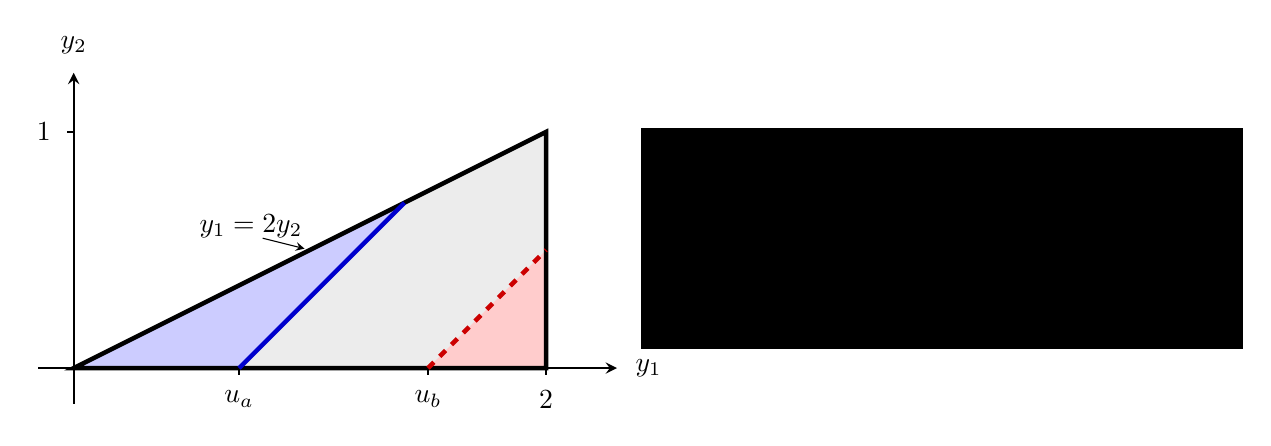
\begin{tikzpicture}[scale=1.5]
    % 1) Backgrounds / Shaded Regions
    \fill[gray!15] (0,0) -- (4,0) -- (4,2) -- cycle;
    \fill[blue!20] (0,0) -- (1.4,0) -- (2.8,1.4) -- cycle;
    \fill[red!20] (3.0,0) -- (4,0) -- (4,1.0) -- cycle;

    % 2) Grid lines and Axes
    \draw[->, thick, >=stealth] (-0.3, 0) -- (4.6, 0) node[right=3pt, black] {$y_1$};
    \draw[->, thick, >=stealth] (0, -0.3) -- (0, 2.5) node[above=3pt, black] {$y_2$};

    % Tick marks
    \draw[thick] (1.4, 0) -- (1.4, -0.06) node[below=2pt, black] {$u_a$};
    \draw[thick] (3.0, 0) -- (3.0, -0.06) node[below=2pt, black] {$u_b$};
    \draw[thick] (4.0, 0) -- (4.0, -0.06) node[below=2pt, black] {$2$};
    \draw[thick] (0, 2.0) -- (-0.06, 2.0) node[left=2pt, black] {$1$};

    % 3) Primary Plots (Support Boundaries and Level Lines)
    \draw[ultra thick, black] (0,0) -- (4,0) -- (4,2) -- cycle;
    \draw[ultra thick, blue!80!black] (1.4, 0) -- (2.8, 1.4);
    \draw[ultra thick, red!80!black, dashed] (3.0, 0) -- (4.0, 1.0);

    % 4) Labels and Callouts
    \node[black] at (1.5, 1.2) {$y_1 = 2y_2$};
    \draw[->, >=stealth, shorten >=2pt] (1.6, 1.1) -- (2.0, 1.0);

    \node[draw, fill=white, align=left, inner sep=7pt, anchor=west, black] at (4.8, 1.1) {
        \textbf{Bivariate Integration Regimes}\\[4pt]
        $\displaystyle \text{Case 1 } (0 \le u_a \le 1): \text{ Blue Triangle } \{U \le u_a\}$\\
        $\displaystyle \text{Vertices: } (0,0),\ (u_a,0),\ (2u_a, u_a)$\\[4pt]
        $\displaystyle \text{Case 2 } (1 < u_b \le 2): \text{ Red Triangle } \{U > u_b\}$\\
        $\displaystyle \text{Vertices: } (u_b,0),\ (2,0),\ (2, 2-u_b)$
    };
\end{tikzpicture}
\end{center}

    \item \textit{Case 1 ($0 \le u \le 1$):} The sublevel set $\{ (y_1, y_2) \in S_{\mathbf{Y}} : y_1 - y_2 \le u \}$ is bounded below by $y_2 = 0$, on the right by $y_1 = y_2 + u$, and on the left by $y_1 = 2y_2$. The lines $y_1 = y_2 + u$ and $y_1 = 2y_2$ intersect at $2y_2 = y_2 + u \implies y_2 = u, y_1 = 2u$. Integrating horizontally first over $2y_2 \le y_1 \le y_2 + u$ and then vertically over $0 \le y_2 \le u$:
    \[
        F_U(u) = \int_{0}^{u} \int_{2y_2}^{y_2 + u} 1\,dy_1\,dy_2 = \int_{0}^{u} (u - y_2)\,dy_2 = \left[ uy_2 - \frac{y_2^2}{2} \right]_{0}^{u} = \frac{u^2}{2}.
    \]
    \item \textit{Case 2 ($1 < u \le 2$):} Using the complement event $\{U > u\} = \{y_1 - y_2 > u\}$, the lower-right corner triangle is bounded by $y_2 = 0$, $y_1 = 2$, and $y_1 = y_2 + u$. These intersect at $(2, 2 - u)$. Thus:
    \[
        F_U(u) = 1 - \Prob(U > u) = 1 - \int_{0}^{2 - u} \int_{y_2 + u}^{2} 1\,dy_1\,dy_2 = 1 - \int_{0}^{2 - u} (2 - u - y_2)\,dy_2 = 1 - \frac{(2 - u)^2}{2}.
    \]
    \item \textit{Summary of CDF and Differentiation:}
    \[
        F_U(u) = \begin{cases} 0, & u < 0, \\ \dfrac{u^2}{2}, & 0 \le u \le 1, \\[6pt] 1 - \dfrac{(2 - u)^2}{2}, & 1 < u \le 2, \\[6pt] 1, & u > 2, \end{cases} \quad \implies \quad f_U(u) = \frac{dF_U(u)}{du} = \begin{cases} u, & 0 \le u \le 1, \\ 2 - u, & 1 < u \le 2, \\ 0, & \text{elsewhere.} \end{cases}
    \]
\end{itemize}

\textbf{Part (b): Expectation $\E(U)$.}
Using the derived triangular density $f_U(u)$:
\[
    \E(U) = \int_{0}^{1} u(u)\,du + \int_{1}^{2} u(2 - u)\,du = \left[ \frac{u^3}{3} \right]_{0}^{1} + \left[ u^2 - \frac{u^3}{3} \right]_{1}^{2} = \frac{1}{3} + \left(4 - \frac{8}{3}\right) - \left(1 - \frac{1}{3}\right) = \frac{1}{3} + \frac{4}{3} - \frac{2}{3} = 1.
\]
Comparing with the bivariate LOTUS method of Chapter 5:
\[
    \E(Y_1 - Y_2) = \int_{0}^{2} \int_{0}^{y_1/2} (y_1 - y_2)\,dy_2\,dy_1 = \int_{0}^{2} \left(\frac{y_1^2}{2} - \frac{y_1^2}{8}\right) dy_1 = \frac{3}{8} \left[\frac{y_1^3}{3}\right]_{0}^{2} = 1.
\]
The results are in complete agreement. \hfill $\blacksquare$

% ----------------------------------------------------------------------------
% EXERCISE 6.7
% ----------------------------------------------------------------------------
\subsection{Exercise 6.7}

\textbf{Original Problem:}
Suppose that $Z$ has a standard normal distribution.
\begin{enumerate}[label=\textbf{\alph*}]
    \item Find the density function of $U = Z^2$.
    \item Does $U$ have a gamma distribution? What are the values of $\alpha$ and $\beta$?
    \item What is another name for the distribution of $U$?
\end{enumerate}

\hrulefill

\textbf{Rigorous Solution:}

\textbf{Part (a): Derivation of $f_U(u)$ for $U = Z^2$.}
Let $Z \sim \mathcal{N}(0, 1)$, with PDF $f_Z(z) = \frac{1}{\sqrt{2\pi}}e^{-z^2/2}$ for all $z \in \R$. Since $Z^2 \ge 0$, $F_U(u) = 0$ for $u \le 0$. For $u > 0$:
\[
    F_U(u) = \Prob(Z^2 \le u) = \Prob(-\sqrt{u} \le Z \le \sqrt{u}) = F_Z(\sqrt{u}) - F_Z(-\sqrt{u}).
\]
Differentiating with respect to $u > 0$ via the Chain Rule and utilizing the even symmetry $f_Z(-\sqrt{u}) = f_Z(\sqrt{u})$:
\begin{align*}
    f_U(u) &= \frac{dF_U(u)}{du} = f_Z(\sqrt{u})\left(\frac{1}{2\sqrt{u}}\right) - f_Z(-\sqrt{u})\left(-\frac{1}{2\sqrt{u}}\right) \\
    &= \frac{1}{2\sqrt{u}} \left[ f_Z(\sqrt{u}) + f_Z(-\sqrt{u}) \right] = \frac{1}{\sqrt{u}} f_Z(\sqrt{u}) = \frac{1}{\sqrt{2\pi}} u^{-1/2} e^{-u/2}.
\end{align*}
Thus,
\[
    f_U(u) = \begin{cases} \dfrac{1}{\sqrt{2\pi}} u^{-1/2} e^{-u/2}, & u > 0, \\[6pt] 0, & \text{elsewhere.} \end{cases}
\]

\textbf{Part (b): Identification as a Gamma Distribution.}
Recall that a $\text{Gamma}(\alpha, \beta)$ random variable has PDF:
\[
    f(u) = \frac{u^{\alpha - 1} e^{-u/\beta}}{\Gamma(\alpha)\beta^\alpha}, \quad u > 0.
\]
Matching exponents in $f_U(u) = \frac{1}{\sqrt{\pi}\cdot 2^{1/2}} u^{1/2 - 1} e^{-u/2}$ and recalling Euler's reflection identity $\Gamma(1/2) = \sqrt{\pi}$, we see that **yes**, $U$ possesses a Gamma distribution with shape parameter $\alpha = \frac{1}{2}$ and scale parameter $\beta = 2$.

\textbf{Part (c): Alternative Name.}
A Gamma distribution with parameters $\alpha = \nu/2$ and $\beta = 2$ is a **Chi-Square distribution** with $\nu$ degrees of freedom. Here $\nu = 1$, so $U$ has a **Chi-Square distribution with $1$ degree of freedom** (denoted $\chi^2(1)$ or $\chi^2_1$). \hfill $\blacksquare$

% ----------------------------------------------------------------------------
% EXERCISE 6.8
% ----------------------------------------------------------------------------
\subsection{Exercise 6.8}

\textbf{Original Problem:}
Assume that $Y$ has a beta distribution with parameters $\alpha$ and $\beta$.
\begin{enumerate}[label=\textbf{\alph*}]
    \item Find the density function of $U = 1 - Y$.
    \item Identify the density of $U$ as one of the types we studied in Chapter 4. Be sure to identify any parameter values.
    \item How is $\E(U)$ related to $\E(Y)$?
    \item How is $V(U)$ related to $V(Y)$?
\end{enumerate}

\hrulefill

\textbf{Rigorous Solution:}

\textbf{Part (a): Derivation of $f_U(u)$.}
The random variable $Y \sim \text{Beta}(\alpha, \beta)$ ($\alpha, \beta > 0$) has PDF:
\[
    f_Y(y) = \begin{cases} \dfrac{y^{\alpha - 1}(1 - y)^{\beta - 1}}{B(\alpha, \beta)}, & 0 \le y \le 1, \\[6pt] 0, & \text{elsewhere,} \end{cases} \qquad \text{where } B(\alpha, \beta) = \frac{\Gamma(\alpha)\Gamma(\beta)}{\Gamma(\alpha + \beta)}.
\]
Since $0 \le Y \le 1$, the reflection $U = 1 - Y$ also has support $S_U = [0, 1]$. For $0 \le u \le 1$:
\[
    F_U(u) = \Prob(1 - Y \le u) = \Prob(Y \ge 1 - u) = 1 - F_Y(1 - u).
\]
Differentiating with respect to $u$ via the Chain Rule and using the symmetry $B(\alpha, \beta) = B(\beta, \alpha)$:
\[
    f_U(u) = \frac{d}{du}\big[1 - F_Y(1 - u)\big] = -f_Y(1 - u)(-1) = f_Y(1 - u) = \begin{cases} \dfrac{u^{\beta - 1}(1 - u)^{\alpha - 1}}{B(\beta, \alpha)}, & 0 \le u \le 1, \\[6pt] 0, & \text{elsewhere.} \end{cases}
\]

\textbf{Part (b): Distribution Identification.}
Comparing $f_U(u)$ with the canonical Beta PDF, $U$ has a **Beta distribution** with swapped parameters: first shape parameter $\alpha^* = \beta$ and second shape parameter $\beta^* = \alpha$, i.e., $U \sim \text{Beta}(\beta, \alpha)$.

\textbf{Part (c): Relationship Between $\E(U)$ and $\E(Y)$.}
By linearity of expectation:
\[
    \E(U) = \E(1 - Y) = 1 - \E(Y) = 1 - \frac{\alpha}{\alpha + \beta} = \frac{\beta}{\alpha + \beta}.
\]

\textbf{Part (d): Relationship Between $V(U)$ and $V(Y)$.}
By the translation-invariance and quadratic scaling property of variance, $V(aY + b) = a^2 V(Y)$:
\[
    V(U) = V(1 - Y) = (-1)^2 V(Y) = V(Y) = \frac{\alpha\beta}{(\alpha + \beta)^2(\alpha + \beta + 1)}. \quad \blacksquare
\]

% ----------------------------------------------------------------------------
% EXERCISE 6.9
% ----------------------------------------------------------------------------
\subsection{Exercise 6.9}

\textbf{Original Problem:}
Suppose that a unit of mineral ore contains a proportion $Y_1$ of metal A and a proportion $Y_2$ of metal B. Experience has shown that the joint probability density function of $Y_1$ and $Y_2$ is uniform over the region $0 \le y_1 \le 1$, $0 \le y_2 \le 1$, $0 \le y_1 + y_2 \le 1$. Let $U = Y_1 + Y_2$, the proportion of either metal A or B per unit. Find
\begin{enumerate}[label=\textbf{\alph*}]
    \item the probability density function for $U$.
    \item $\E(U)$ by using the answer to part (a).
    \item $\E(U)$ by using only the marginal densities of $Y_1$ and $Y_2$.
\end{enumerate}

\hrulefill

\textbf{Rigorous Solution:}

\textbf{Preliminary Normalization:} The support region $S_{\mathbf{Y}} = \{(y_1, y_2) : y_1 \ge 0, y_2 \ge 0, y_1 + y_2 \le 1\}$ is the standard $2$-simplex (a right triangle of base $1$ and height $1$), whose Euclidean area is $\text{Area}(S_{\mathbf{Y}}) = \frac{1}{2}(1)(1) = \frac{1}{2}$. Because the joint distribution is uniform over $S_{\mathbf{Y}}$, the constant density height must be $f(y_1, y_2) = \frac{1}{\text{Area}(S_{\mathbf{Y}})} = 2$ on $S_{\mathbf{Y}}$, and $0$ elsewhere.

\textbf{Part (a): Derivation of $f_U(u)$.}
\begin{itemize}
    \item Since $0 \le y_1 + y_2 \le 1$ on $S_{\mathbf{Y}}$, the support of $U = Y_1 + Y_2$ is $[0, 1]$.
    \item For $u < 0$, $F_U(u) = 0$; for $u > 1$, $F_U(u) = 1$.
    \item For $0 \le u \le 1$, the region $\{(y_1, y_2) \in S_{\mathbf{Y}} : y_1 + y_2 \le u\}$ is a right triangle with vertices $(0,0)$, $(u,0)$, and $(0,u)$ completely contained within $S_{\mathbf{Y}}$:
    \[
        F_U(u) = \Prob(Y_1 + Y_2 \le u) = \int_{0}^{u} \int_{0}^{u - y_1} 2\,dy_2\,dy_1 = \int_{0}^{u} 2(u - y_1)\,dy_1 = \Big[ -(u - y_1)^2 \Big]_{0}^{u} = u^2.
    \]
    \item Differentiating with respect to $u$ yields:
    \[
        f_U(u) = \frac{dF_U(u)}{du} = \begin{cases} 2u, & 0 \le u \le 1, \\ 0, & \text{elsewhere.} \end{cases}
    \]
\end{itemize}

\textbf{Part (b): $\E(U)$ via $f_U(u)$.}
\[
    \E(U) = \int_{0}^{1} u(2u)\,du = \left[ \frac{2u^3}{3} \right]_{0}^{1} = \frac{2}{3}.
\]

\textbf{Part (c): $\E(U)$ via Marginal Densities.}
For $0 \le y_1 \le 1$, the marginal density of $Y_1$ is obtained by integrating out $y_2 \in [0, 1 - y_1]$:
\[
    f_1(y_1) = \int_{0}^{1 - y_1} 2\,dy_2 = 2(1 - y_1), \quad 0 \le y_1 \le 1.
\]
By symmetry of $f(y_1, y_2)$ and $S_{\mathbf{Y}}$ with respect to $y_1$ and $y_2$, the marginal density of $Y_2$ is $f_2(y_2) = 2(1 - y_2)$ for $0 \le y_2 \le 1$. Computing the marginal expectations:
\[
    \E(Y_1) = \E(Y_2) = \int_{0}^{1} 2y_1(1 - y_1)\,dy_1 = 2\left(\frac{1}{2} - \frac{1}{3}\right) = \frac{1}{3}.
\]
Therefore, $\E(U) = \E(Y_1) + \E(Y_2) = \frac{1}{3} + \frac{1}{3} = \frac{2}{3}$. \hfill $\blacksquare$

% ----------------------------------------------------------------------------
% EXERCISE 6.10
% ----------------------------------------------------------------------------
\subsection{Exercise 6.10}

\textbf{Original Problem:}
The total time from arrival to completion of service at a fast-food outlet, $Y_1$, and the time spent waiting in line before arriving at the service window, $Y_2$, were given in Exercise 5.15 with joint density function
\[
    f(y_1, y_2) = \begin{cases} e^{-y_1}, & 0 \le y_2 \le y_1 < \infty, \\ 0, & \text{elsewhere.} \end{cases}
\]
Another random variable of interest is $U = Y_1 - Y_2$, the time spent at the service window. Find
\begin{enumerate}[label=\textbf{\alph*}]
    \item the probability density function for $U$.
    \item $\E(U)$ and $V(U)$. Compare your answers with the results of Exercise 5.108.
\end{enumerate}

\hrulefill

\textbf{Rigorous Solution:}

\textbf{Part (a): Derivation of $f_U(u)$.}
\begin{itemize}
    \item \textit{Support:} Since $0 \le y_2 \le y_1 < \infty$, the difference $U = Y_1 - Y_2$ satisfies $U \ge 0$ almost surely. Thus $F_U(u) = 0$ for $u < 0$.
    \item \textit{CDF for $u \ge 0$:} The event $\{U > u\} = \{Y_1 - Y_2 > u\} = \{Y_1 > Y_2 + u\}$ in the octant $0 \le y_2 \le y_1 < \infty$ corresponds to $0 \le y_2 < \infty$ and $y_2 + u < y_1 < \infty$. Integrating over this complementary region via Tonelli's Theorem:
    \begin{align*}
        F_U(u) &= 1 - \Prob(Y_1 - Y_2 > u) = 1 - \int_{0}^{\infty} \int_{y_2 + u}^{\infty} e^{-y_1}\,dy_1\,dy_2 \\
        &= 1 - \int_{0}^{\infty} \Big[ -e^{-y_1} \Big]_{y_2 + u}^{\infty} dy_2 = 1 - \int_{0}^{\infty} e^{-(y_2 + u)}\,dy_2 \\
        &= 1 - e^{-u} \int_{0}^{\infty} e^{-y_2}\,dy_2 = 1 - e^{-u}(1) = 1 - e^{-u}.
    \end{align*}
    \item \textit{PDF:} Differentiating $F_U(u)$ with respect to $u$:
    \[
        f_U(u) = \frac{dF_U(u)}{du} = \begin{cases} e^{-u}, & u \ge 0, \\ 0, & \text{elsewhere.} \end{cases}
    \]
    Hence, $U \sim \text{Exponential}(\beta = 1)$.
\end{itemize}

\textbf{Part (b): Expectation and Variance.}
Because $U$ follows an Exponential distribution with scale parameter $\beta = 1$:
\[
    \E(U) = \beta = 1, \qquad V(U) = \beta^2 = 1^2 = 1.
\]
This matches the bivariate covariance calculations of Chapter 5 (where $\E(Y_1) = 2$, $\E(Y_2) = 1$, $V(Y_1) = 2$, $V(Y_2) = 1$, and $\text{Cov}(Y_1, Y_2) = 1$, giving $V(Y_1 - Y_2) = 2 + 1 - 2(1) = 1$). \hfill $\blacksquare$

% ----------------------------------------------------------------------------
% EXERCISE 6.11
% ----------------------------------------------------------------------------
\subsection{Exercise 6.11}

\textbf{Original Problem:}
Suppose that two electronic components in the guidance system for a missile operate independently and that each has a length of life governed by the exponential distribution with mean $1$ (with measurements in hundreds of hours). Find the
\begin{enumerate}[label=\textbf{\alph*}]
    \item probability density function for the average length of life of the two components.
    \item mean and variance of this average, using the answer in part (a). Check your answer by computing the mean and variance, using Theorem 5.12.
\end{enumerate}

\hrulefill

\textbf{Rigorous Solution:}

\textbf{Part (a): Derivation of $f_U(u)$ for $U = \frac{Y_1 + Y_2}{2}$.}
Since $Y_1, Y_2 \stackrel{\text{i.i.d.}}{\sim} \text{Exponential}(1)$, their joint PDF is:
\[
    f(y_1, y_2) = f_1(y_1)f_2(y_2) = \begin{cases} e^{-(y_1 + y_2)}, & y_1 \ge 0, \ y_2 \ge 0, \\ 0, & \text{elsewhere.} \end{cases}
\]
For $u < 0$, $F_U(u) = 0$. For $u \ge 0$, the event $\{U \le u\} = \left\{\frac{Y_1 + Y_2}{2} \le u\right\} = \{Y_1 + Y_2 \le 2u\}$ is the triangle in the first quadrant bounded by $y_1 = 0$, $y_2 = 0$, and $y_1 + y_2 = 2u$:
\begin{align*}
    F_U(u) &= \int_{0}^{2u} \int_{0}^{2u - y_1} e^{-y_1} e^{-y_2}\,dy_2\,dy_1 = \int_{0}^{2u} e^{-y_1} \left(1 - e^{-(2u - y_1)}\right) dy_1 \\
    &= \int_{0}^{2u} \left(e^{-y_1} - e^{-2u}\right) dy_1 = \Big[ -e^{-y_1} - y_1 e^{-2u} \Big]_{0}^{2u} = 1 - e^{-2u} - 2u e^{-2u}.
\end{align*}
Differentiating with respect to $u \ge 0$ via the Product Rule:
\[
    f_U(u) = \frac{dF_U(u)}{du} = 2e^{-2u} - \left(2e^{-2u} - 4u e^{-2u}\right) = 4u e^{-2u}.
\]
Thus,
\[
    f_U(u) = \begin{cases} 4u e^{-2u}, & u \ge 0, \\ 0, & \text{elsewhere.} \end{cases}
\]

\textbf{Part (b): Mean and Variance Verification.}
Observing that $f_U(u) = \frac{u^{2 - 1} e^{-u/(1/2)}}{\Gamma(2)(1/2)^2}$ is a $\text{Gamma}\left(\alpha = 2, \beta = \frac{1}{2}\right)$ density (or integrating by parts directly):
\[
    \E(U) = \alpha\beta = 2\left(\frac{1}{2}\right) = 1, \qquad V(U) = \alpha\beta^2 = 2\left(\frac{1}{2}\right)^2 = \frac{1}{2}.
\]
Checking via Theorem 5.12 (Linear Combinations of Independent Random Variables), since $\E(Y_i) = 1$ and $V(Y_i) = 1$ for $i = 1, 2$ with $\text{Cov}(Y_1, Y_2) = 0$:
\[
    \E\left(\frac{1}{2}Y_1 + \frac{1}{2}Y_2\right) = \frac{1}{2}(1) + \frac{1}{2}(1) = 1, \qquad V\left(\frac{1}{2}Y_1 + \frac{1}{2}Y_2\right) = \left(\frac{1}{2}\right)^2 V(Y_1) + \left(\frac{1}{2}\right)^2 V(Y_2) = \frac{1}{4} + \frac{1}{4} = \frac{1}{2}. \quad \blacksquare
\]

% ----------------------------------------------------------------------------
% EXERCISE 6.12
% ----------------------------------------------------------------------------
\subsection{Exercise 6.12}

\textbf{Original Problem:}
Suppose that $Y$ has a gamma distribution with parameters $\alpha$ and $\beta$ and that $c > 0$ is a constant.
\begin{enumerate}[label=\textbf{\alph*}]
    \item Derive the density function of $U = cY$.
    \item Identify the density of $U$ as one of the types we studied in Chapter 4. Be sure to identify any parameter values.
    \item The parameters $\alpha$ and $\beta$ of a gamma-distributed random variable are, respectively, ``shape'' and ``scale'' parameters. How do the scale and shape parameters for $U$ compare to those for $Y$?
\end{enumerate}

\hrulefill

\textbf{Rigorous Solution:}

\textbf{Part (a): Derivation of $f_U(u)$.}
Let $Y \sim \text{Gamma}(\alpha, \beta)$ with PDF $f_Y(y) = \frac{y^{\alpha - 1} e^{-y/\beta}}{\Gamma(\alpha)\beta^\alpha}$ for $y > 0$, and $0$ elsewhere. Since $c > 0$, $U = cY > 0$ almost surely. For $u > 0$:
\[
    F_U(u) = \Prob(cY \le u) = \Prob\left(Y \le \frac{u}{c}\right) = F_Y\left(\frac{u}{c}\right) = \int_{0}^{u/c} \frac{y^{\alpha - 1} e^{-y/\beta}}{\Gamma(\alpha)\beta^\alpha}\,dy.
\]
Differentiating with respect to $u$ via the Fundamental Theorem of Calculus and Chain Rule:
\[
    f_U(u) = \frac{dF_U(u)}{du} = f_Y\left(\frac{u}{c}\right) \cdot \frac{1}{c} = \frac{(u/c)^{\alpha - 1} e^{-(u/c)/\beta}}{\Gamma(\alpha)\beta^\alpha} \cdot \frac{1}{c} = \frac{u^{\alpha - 1} e^{-u/(c\beta)}}{\Gamma(\alpha)(c\beta)^\alpha}, \quad u > 0,
\]
and $f_U(u) = 0$ for $u \le 0$.

\textbf{Part (b): Distribution Identification.}
Comparing $f_U(u)$ to the standard Gamma PDF, $U$ has a **Gamma distribution** with shape parameter $\alpha^* = \alpha$ and scale parameter $\beta^* = c\beta$, i.e., $U \sim \text{Gamma}(\alpha, c\beta)$.

\textbf{Part (c): Comparison of Shape and Scale Parameters.}
Under positive linear rescaling $U = cY$, the **shape parameter remains invariant** ($\alpha^* = \alpha$), preserving the skewness and morphological profile of the distribution, whereas the **scale parameter is multiplied by $c$** ($\beta^* = c\beta$), stretching or compressing the horizontal axis proportionally. \hfill $\blacksquare$

% ----------------------------------------------------------------------------
% EXERCISE 6.13
% ----------------------------------------------------------------------------
\subsection{Exercise 6.13}

\textbf{Original Problem:}
If $Y_1$ and $Y_2$ are independent exponential random variables, both with mean $\beta$, find the density function for their sum. (In Exercise 5.7, we considered two independent exponential random variables, both with mean $1$ and determined $P(Y_1 + Y_2 \le 3)$.)

\hrulefill

\textbf{Rigorous Solution:}

Let $Y_1, Y_2 \stackrel{\text{i.i.d.}}{\sim} \text{Exponential}(\beta)$ ($\beta > 0$). By independence, their joint density is:
\[
    f(y_1, y_2) = \begin{cases} \dfrac{1}{\beta^2} e^{-(y_1 + y_2)/\beta}, & y_1 \ge 0, \ y_2 \ge 0, \\[6pt] 0, & \text{elsewhere.} \end{cases}
\]
Let $U = Y_1 + Y_2$. For $u < 0$, $F_U(u) = 0$. For $u \ge 0$, integrating over the simplex $\{y_1 \ge 0, y_2 \ge 0 : y_1 + y_2 \le u\}$:
\begin{align*}
    F_U(u) &= \Prob(Y_1 + Y_2 \le u) = \int_{0}^{u} \int_{0}^{u - y_1} \frac{1}{\beta^2} e^{-(y_1 + y_2)/\beta}\,dy_2\,dy_1 \\
    &= \frac{1}{\beta} \int_{0}^{u} e^{-y_1/\beta} \left[ -e^{-y_2/\beta} \right]_{0}^{u - y_1} dy_1 = \frac{1}{\beta} \int_{0}^{u} \left(e^{-y_1/\beta} - e^{-u/\beta}\right) dy_1 \\
    &= \left[ -e^{-y_1/\beta} - \frac{y_1}{\beta}e^{-u/\beta} \right]_{0}^{u} = 1 - e^{-u/\beta} - \frac{u}{\beta}e^{-u/\beta}.
\end{align*}
Differentiating $F_U(u)$ with respect to $u \ge 0$:
\[
    f_U(u) = \frac{dF_U(u)}{du} = \frac{1}{\beta}e^{-u/\beta} - \left(\frac{1}{\beta}e^{-u/\beta} - \frac{u}{\beta^2}e^{-u/\beta}\right) = \frac{u}{\beta^2}e^{-u/\beta}.
\]
Thus, the PDF of the sum $U = Y_1 + Y_2$ is:
\[
    f_U(u) = \begin{cases} \dfrac{u}{\beta^2}e^{-u/\beta}, & u \ge 0, \\[6pt] 0, & \text{elsewhere,} \end{cases}
\]
which is a $\text{Gamma}(2, \beta)$ (or $\text{Erlang}(2, \beta)$) distribution. \hfill $\blacksquare$

% ----------------------------------------------------------------------------
% EXERCISE 6.14
% ----------------------------------------------------------------------------
\subsection{Exercise 6.14}

\textbf{Original Problem:}
In a process of sintering (heating) two types of copper powder (see Exercise 5.152), the density function for $Y_1$, the volume proportion of solid copper in a sample, was given by
\[
    f_1(y_1) = \begin{cases} 6y_1(1 - y_1), & 0 \le y_1 \le 1, \\ 0, & \text{elsewhere.} \end{cases}
\]
The density function for $Y_2$, the proportion of type A crystals among the solid copper, was given as
\[
    f_2(y_2) = \begin{cases} 3y_2^2, & 0 \le y_2 \le 1, \\ 0, & \text{elsewhere.} \end{cases}
\]
The variable $U = Y_1 Y_2$ gives the proportion of the sample volume due to type A crystals. If $Y_1$ and $Y_2$ are independent, find the probability density function for $U$.

\hrulefill

\textbf{Rigorous Solution:}

\begin{itemize}
    \item \textit{Joint Density and Support:} By independence, the joint density on the unit square $[0, 1]^2$ is:
    \[
        f(y_1, y_2) = f_1(y_1)f_2(y_2) = 18y_1(1 - y_1)y_2^2, \quad 0 \le y_1 \le 1, \ 0 \le y_2 \le 1.
    \]
    Since $Y_1, Y_2 \in [0, 1]$, the product $U = Y_1 Y_2$ has support $S_U = [0, 1]$. For $u \le 0$, $F_U(u) = 0$; for $u > 1$, $F_U(u) = 1$.

\begin{center}
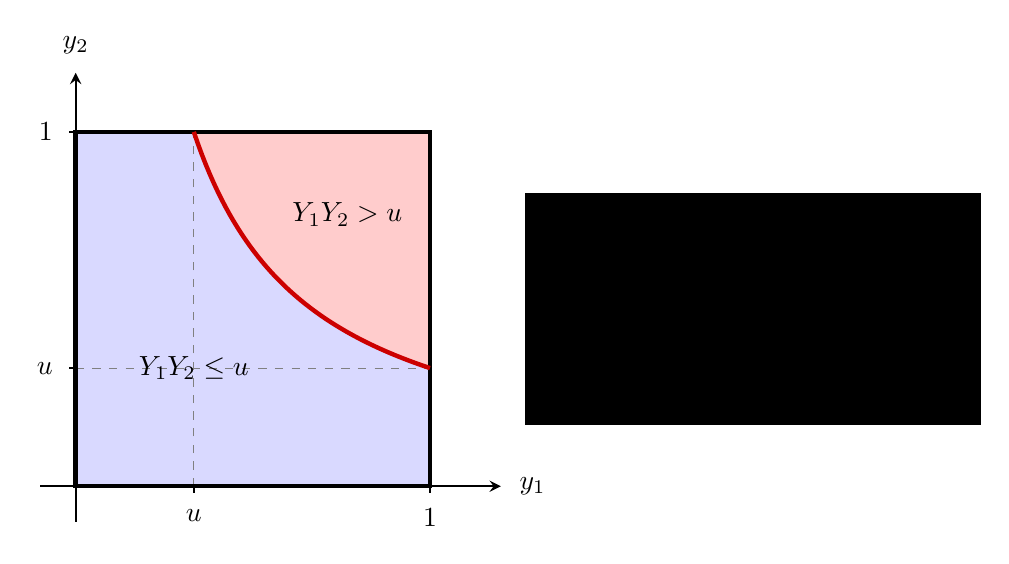
\begin{tikzpicture}[scale=1.5]
    % 1) Backgrounds / Shaded Regions
    \fill[blue!15] (0,0) -- (3,0) -- (3,1.0) -- plot[domain=3:1.0, samples=50] (\x, {3.0/\x}) -- (0,3) -- cycle;
    \fill[red!20] (1.0,3) -- (3,3) -- (3,1.0) -- plot[domain=3:1.0, samples=50] (\x, {3.0/\x}) -- cycle;

    % 2) Grid lines and Axes
    \draw[->, thick, >=stealth] (-0.3, 0) -- (3.6, 0) node[right=3pt, black] {$y_1$};
    \draw[->, thick, >=stealth] (0, -0.3) -- (0, 3.5) node[above=3pt, black] {$y_2$};

    % Tick marks
    \draw[thick] (1.0, 0) -- (1.0, -0.06) node[below=2pt, black] {$u$};
    \draw[thick] (3.0, 0) -- (3.0, -0.06) node[below=2pt, black] {$1$};
    \draw[thick] (0, 1.0) -- (-0.06, 1.0) node[left=2pt, black] {$u$};
    \draw[thick] (0, 3.0) -- (-0.06, 3.0) node[left=2pt, black] {$1$};
    \draw[dashed, gray] (1.0, 0) -- (1.0, 3.0);
    \draw[dashed, gray] (0, 1.0) -- (3.0, 1.0);

    % 3) Primary Plots
    \draw[ultra thick, black] (0,0) rectangle (3,3);
    \draw[ultra thick, red!80!black, domain=1.0:3.0, samples=60] plot (\x, {3.0/\x});

    % 4) Labels and Callouts
    \node[black] at (2.3, 2.3) {$Y_1 Y_2 > u$};
    \node[black] at (1.0, 1.0) {$Y_1 Y_2 \le u$};

    \node[draw, fill=white, align=left, inner sep=7pt, anchor=west, black] at (3.8, 1.5) {
        \textbf{Hyperbolic Sublevel Partition}\\[4pt]
        $\displaystyle \text{Boundary Curve: } y_2 = \frac{u}{y_1}$\\[4pt]
        $\displaystyle \text{Red Upper Region } \{Y_1 Y_2 > u\}:$\\
        $\displaystyle u \le y_1 \le 1, \quad \frac{u}{y_1} \le y_2 \le 1$
    };
\end{tikzpicture}
\end{center}

    \item \textit{CDF via Complementary Hyperbolic Region:} For $0 < u \le 1$, the level curve $y_1 y_2 = u$ is the rectangular hyperbola $y_2 = \frac{u}{y_1}$, which enters the top of the unit square at $(u, 1)$ and exits the right side at $(1, u)$. The upper-right complementary region $\{Y_1 Y_2 > u\}$ is given by $u \le y_1 \le 1$ and $\frac{u}{y_1} \le y_2 \le 1$. Therefore:
    \begin{align*}
        F_U(u) &= 1 - \Prob(Y_1 Y_2 > u) = 1 - \int_{u}^{1} \int_{u/y_1}^{1} 6y_1(1 - y_1) \cdot 3y_2^2\,dy_2\,dy_1 \\
        &= 1 - \int_{u}^{1} 6y_1(1 - y_1) \Big[ y_2^3 \Big]_{u/y_1}^{1} dy_1 \\
        &= 1 - 6 \int_{u}^{1} y_1(1 - y_1)\left(1 - \frac{u^3}{y_1^3}\right) dy_1 \\
        &= 1 - 6 \int_{u}^{1} \left(y_1 - y_1^2 - u^3 y_1^{-2} + u^3 y_1^{-1}\right) dy_1 \\
        &= 1 - 6 \left[ \frac{y_1^2}{2} - \frac{y_1^3}{3} + u^3 y_1^{-1} + u^3 \ln y_1 \right]_{u}^{1} \\
        &= 1 - 6 \left[ \left(\frac{1}{2} - \frac{1}{3} + u^3 + 0\right) - \left(\frac{u^2}{2} - \frac{u^3}{3} + u^2 + u^3 \ln u\right) \right] \\
        &= 1 - 6 \left( \frac{1}{6} - \frac{3}{2}u^2 + \frac{4}{3}u^3 - u^3 \ln u \right) \\
        &= 9u^2 - 8u^3 + 6u^3 \ln u.
    \end{align*}
    \item \textit{Differentiation (or Leibniz Rule):} Differentiating $F_U(u)$ with respect to $u \in (0, 1]$:
    \[
        f_U(u) = \frac{dF_U(u)}{du} = 18u - 24u^2 + 18u^2 \ln u + 6u^3\left(\frac{1}{u}\right) = 18u - 18u^2 + 18u^2 \ln u.
    \]
    Factoring out $18u$ yields the final density:
    \[
        f_U(u) = \begin{cases} 18u(1 - u + u\ln u), & 0 < u \le 1, \\ 0, & \text{elsewhere.} \end{cases} \quad \blacksquare
    \]
\end{itemize}

% ----------------------------------------------------------------------------
% EXERCISE 6.15
% ----------------------------------------------------------------------------
\subsection{Exercise 6.15}

\textbf{Original Problem:}
Let $Y$ have a distribution function given by
\[
    F(y) = \begin{cases} 0, & y < 0, \\ 1 - e^{-y^2}, & y \ge 0. \end{cases}
\]
Find a transformation $G(U)$ such that, if $U$ has a uniform distribution on the interval $(0, 1)$, $G(U)$ has the same distribution as $Y$.

\hrulefill

\textbf{Rigorous Solution:}

\textbf{Proof Technique:} Quantile Inversion Method (Theorem 1.4).
\begin{itemize}
    \item Observe that on the support $[0, \infty)$, $F(y) = 1 - e^{-y^2}$ has derivative $F'(y) = 2y e^{-y^2} > 0$ for all $y > 0$, and maps $(0, \infty)$ bijectively onto $(0, 1)$.
    \item For any $u \in (0, 1)$, we solve $F(y) = u$ uniquely for $y > 0$:
    \[
        1 - e^{-y^2} = u \iff e^{-y^2} = 1 - u \iff -y^2 = \ln(1 - u) \iff y = \sqrt{-\ln(1 - u)}.
    \]
    \item Define the transformation $G(U) = F^{-1}(U) = \sqrt{-\ln(1 - U)}$. Let us rigorously verify that $G(U)$ has CDF $F(y)$:
    \begin{itemize}
        \item For $y < 0$, since $\sqrt{-\ln(1 - U)} > 0$ almost surely, $\Prob(G(U) \le y) = 0 = F(y)$.
        \item For $y \ge 0$, using the fact that $0 < 1 - e^{-y^2} < 1$ for $y > 0$ and $F_U(u) = u$ on $(0, 1)$:
        \begin{align*}
            \Prob(G(U) \le y) &= \Prob\left(\sqrt{-\ln(1 - U)} \le y\right) = \Prob\left(-\ln(1 - U) \le y^2\right) \\
            &= \Prob\left(\ln(1 - U) \ge -y^2\right) = \Prob\left(1 - U \ge e^{-y^2}\right) \\
            &= \Prob\left(U \le 1 - e^{-y^2}\right) = 1 - e^{-y^2} = F(y).
        \end{align*}
    \end{itemize}
\end{itemize}
Thus, $G(U) = \sqrt{-\ln(1 - U)}$ (or equivalently $\sqrt{-\ln U}$, since $1 - U \stackrel{d}{=} U$) possesses the distribution of $Y$. \hfill $\blacksquare$

% ----------------------------------------------------------------------------
% EXERCISE 6.16
% ----------------------------------------------------------------------------
\subsection{Exercise 6.16}

\textbf{Original Problem:}
In Exercise 4.15, we determined that
\[
    f(y) = \begin{cases} \dfrac{b}{y^2}, & y \ge b, \\[6pt] 0, & \text{elsewhere,} \end{cases}
\]
is a bona fide probability density function for a random variable, $Y$. Assuming $b$ is a known constant and $U$ has a uniform distribution on the interval $(0, 1)$, transform $U$ to obtain a random variable with the same distribution as $Y$.

\hrulefill

\textbf{Rigorous Solution:}

Note that for $f(y)$ to be a valid PDF on $[b, \infty)$, we must have $b > 0$.
\begin{enumerate}
    \item \textit{Derivation of the CDF $F_Y(y)$:} For $y < b$, $F_Y(y) = 0$. For $y \ge b$:
    \[
        F_Y(y) = \int_{b}^{y} \frac{b}{t^2}\,dt = \left[ -\frac{b}{t} \right]_{b}^{y} = -\frac{b}{y} - \left(-\frac{b}{b}\right) = 1 - \frac{b}{y}.
    \]
    \item \textit{Quantile Inversion:} On $[b, \infty)$, $F_Y(y) = 1 - \frac{b}{y}$ is strictly increasing and maps $[b, \infty)$ onto $[0, 1)$. For $u \in (0, 1)$, setting $F_Y(y) = u$:
    \[
        1 - \frac{b}{y} = u \iff \frac{b}{y} = 1 - u \iff y = \frac{b}{1 - u}.
    \]
    \item \textit{Verification:} Define $G(U) = \frac{b}{1 - U}$. For any $y \ge b$, we have $0 \le 1 - \frac{b}{y} < 1$, and:
    \[
        \Prob\left(\frac{b}{1 - U} \le y\right) = \Prob\left(1 - U \ge \frac{b}{y}\right) = \Prob\left(U \le 1 - \frac{b}{y}\right) = 1 - \frac{b}{y} = F_Y(y).
    \]
\end{enumerate}
Hence, the required transformation is $G(U) = \dfrac{b}{1 - U}$ (or $G(U) = \dfrac{b}{U}$). \hfill $\blacksquare$

% ----------------------------------------------------------------------------
% EXERCISE 6.17
% ----------------------------------------------------------------------------
\subsection{Exercise 6.17}

\textbf{Original Problem:}
A member of the power family of distributions has a distribution function given by
\[
    F(y) = \begin{cases} 0, & y < 0, \\ \left(\dfrac{y}{\theta}\right)^\alpha, & 0 \le y \le \theta, \\[8pt] 1, & y > \theta, \end{cases}
\]
where $\alpha, \theta > 0$.
\begin{enumerate}[label=\textbf{\alph*}]
    \item Find the density function.
    \item For fixed values of $\alpha$ and $\theta$, find a transformation $G(U)$ so that $G(U)$ has a distribution function of $F$ when $U$ possesses a uniform $(0, 1)$ distribution.
    \item Given that a random sample of size $5$ from a uniform distribution on the interval $(0, 1)$ yielded the values $.2700$, $.6901$, $.1413$, $.1523$, and $.3609$, use the transformation derived in part (b) to give values associated with a random variable with a power family distribution with $\alpha = 2, \theta = 4$.
\end{enumerate}

\hrulefill

\textbf{Rigorous Solution:}

\textbf{Part (a): Density Function.}
Differentiating $F(y)$ with respect to $y$ on the open interval $(0, \theta)$:
\[
    f(y) = \frac{dF(y)}{dy} = \begin{cases} \dfrac{\alpha y^{\alpha - 1}}{\theta^\alpha}, & 0 < y \le \theta, \\[6pt] 0, & \text{elsewhere.} \end{cases}
\]

\textbf{Part (b): Inverse Transformation $G(U)$.}
For $u \in (0, 1)$ and $y \in (0, \theta)$, solving $F(y) = u$:
\[
    \left(\frac{y}{\theta}\right)^\alpha = u \iff \frac{y}{\theta} = u^{1/\alpha} \iff y = \theta u^{1/\alpha}.
\]
Thus, $G(U) = \theta U^{1/\alpha}$. Indeed, for $0 \le y \le \theta$:
\[
    \Prob(\theta U^{1/\alpha} \le y) = \Prob\left(U \le \left(\frac{y}{\theta}\right)^\alpha\right) = \left(\frac{y}{\theta}\right)^\alpha = F(y).
\]

\textbf{Part (c): Numerical Simulation for $\alpha = 2, \theta = 4$.}
Substituting $\alpha = 2$ and $\theta = 4$ into $G(u) = \theta u^{1/\alpha}$ gives $G(u) = 4\sqrt{u}$:
\begin{itemize}
    \item $u_1 = 0.2700 \implies y_1 = 4\sqrt{0.2700} \approx 4(0.519615) \approx 2.0785$.
    \item $u_2 = 0.6901 \implies y_2 = 4\sqrt{0.6901} \approx 4(0.830723) \approx 3.3229$.
    \item $u_3 = 0.1413 \implies y_3 = 4\sqrt{0.1413} \approx 4(0.375899) \approx 1.5036$.
    \item $u_4 = 0.1523 \implies y_4 = 4\sqrt{0.1523} \approx 4(0.390256) \approx 1.5610$.
    \item $u_5 = 0.3609 \implies y_5 = 4\sqrt{0.3609} \approx 4(0.600750) \approx 2.4030$. \hfill $\blacksquare$
\end{itemize}

% ----------------------------------------------------------------------------
% EXERCISE 6.18
% ----------------------------------------------------------------------------
\subsection{Exercise 6.18}

\textbf{Original Problem:}
A member of the Pareto family of distributions (often used in economics to model income distributions) has a distribution function given by
\[
    F(y) = \begin{cases} 0, & y < \beta, \\ 1 - \left(\dfrac{\beta}{y}\right)^\alpha, & y \ge \beta, \end{cases}
\]
where $\alpha, \beta > 0$.
\begin{enumerate}[label=\textbf{\alph*}]
    \item Find the density function.
    \item For fixed values of $\beta$ and $\alpha$, find a transformation $G(U)$ so that $G(U)$ has a distribution function of $F$ when $U$ has a uniform distribution on the interval $(0, 1)$.
    \item Given that a random sample of size $5$ from a uniform distribution on the interval $(0, 1)$ yielded the values $.0058$, $.2048$, $.7692$, $.2475$ and $.6078$, use the transformation derived in part (b) to give values associated with a random variable with a Pareto distribution with $\alpha = 2, \beta = 3$.
\end{enumerate}

\hrulefill

\textbf{Rigorous Solution:}

\textbf{Part (a): Density Function.}
Differentiating $F(y) = 1 - \beta^\alpha y^{-\alpha}$ with respect to $y$ for $y \ge \beta$:
\[
    f(y) = \frac{dF(y)}{dy} = \begin{cases} \dfrac{\alpha \beta^\alpha}{y^{\alpha + 1}}, & y \ge \beta, \\[6pt] 0, & \text{elsewhere.} \end{cases}
\]

\textbf{Part (b): Inverse Transformation $G(U)$.}
For $u \in (0, 1)$ and $y \ge \beta$, solving $F(y) = u$:
\[
    1 - \left(\frac{\beta}{y}\right)^\alpha = u \iff \left(\frac{\beta}{y}\right)^\alpha = 1 - u \iff \frac{\beta}{y} = (1 - u)^{1/\alpha} \iff y = \beta(1 - u)^{-1/\alpha}.
\]
Thus, $G(U) = \beta(1 - U)^{-1/\alpha}$. For any $y \ge \beta$:
\[
    \Prob\left(\beta(1 - U)^{-1/\alpha} \le y\right) = \Prob\left(1 - U \ge \left(\frac{\beta}{y}\right)^\alpha\right) = \Prob\left(U \le 1 - \left(\frac{\beta}{y}\right)^\alpha\right) = 1 - \left(\frac{\beta}{y}\right)^\alpha = F(y).
\]

\textbf{Part (c): Numerical Simulation for $\alpha = 2, \beta = 3$.}
Substituting $\alpha = 2$ and $\beta = 3$ yields $G(u) = \dfrac{3}{\sqrt{1 - u}}$:
\begin{itemize}
    \item $u_1 = 0.0058 \implies y_1 = \dfrac{3}{\sqrt{1 - 0.0058}} = \dfrac{3}{\sqrt{0.9942}} \approx 3.0087$.
    \item $u_2 = 0.2048 \implies y_2 = \dfrac{3}{\sqrt{1 - 0.2048}} = \dfrac{3}{\sqrt{0.7952}} \approx 3.3642$.
    \item $u_3 = 0.7692 \implies y_3 = \dfrac{3}{\sqrt{1 - 0.7692}} = \dfrac{3}{\sqrt{0.2308}} \approx 6.2446$.
    \item $u_4 = 0.2475 \implies y_4 = \dfrac{3}{\sqrt{1 - 0.2475}} = \dfrac{3}{\sqrt{0.7525}} \approx 3.4583$.
    \item $u_5 = 0.6078 \implies y_5 = \dfrac{3}{\sqrt{1 - 0.6078}} = \dfrac{3}{\sqrt{0.3922}} \approx 4.7903$. \hfill $\blacksquare$
\end{itemize}

% ----------------------------------------------------------------------------
% EXERCISE 6.19
% ----------------------------------------------------------------------------
\subsection{Exercise 6.19}

\textbf{Original Problem:}
Refer to Exercises 6.17 and 6.18. If $Y$ possesses a Pareto distribution with parameters $\alpha$ and $\beta$, prove that $X = 1/Y$ has a power family distribution with parameters $\alpha$ and $\theta = \beta^{-1}$.

\hrulefill

\textbf{Rigorous Solution:}

\begin{proof}[Direct Proof via the Method of Distribution Functions]
Let $Y \sim \text{Pareto}(\alpha, \beta)$ with $\alpha, \beta > 0$. By Exercise 6.18, $Y$ is a continuous random variable supported on $[\beta, \infty)$ with cumulative distribution function:
\[
    F_Y(y) = 1 - \left(\frac{\beta}{y}\right)^\alpha, \quad y \ge \beta,
\]
and $F_Y(y) = 0$ for $y < \beta$. Consider the reciprocal random variable $X = \frac{1}{Y}$.
\begin{enumerate}
    \item \textit{Support Analysis:} Because $Y \ge \beta > 0$ with probability $1$, the reciprocal $X = 1/Y$ satisfies $0 < X \le \frac{1}{\beta} = \beta^{-1}$ with probability $1$. Let $\theta \coloneqq \beta^{-1} > 0$.
    \begin{itemize}
        \item For $x \le 0$: Since $X > 0$ almost surely, $F_X(x) = \Prob(X \le x) = 0$.
        \item For $x > \theta = \beta^{-1}$: Since $X \le \beta^{-1}$ almost surely, $F_X(x) = \Prob(X \le x) = 1$.
    \end{itemize}
    \item \textit{Interior Distribution ($0 < x \le \theta = \beta^{-1}$):} Since $x > 0$ and $Y > 0$, taking reciprocals reverses the inequality:
    \[
        F_X(x) = \Prob(X \le x) = \Prob\left(\frac{1}{Y} \le x\right) = \Prob\left(Y \ge \frac{1}{x}\right).
    \]
    Because $Y$ is an absolutely continuous random variable, $\Prob(Y = 1/x) = 0$. Moreover, $0 < x \le \beta^{-1}$ implies $\frac{1}{x} \ge \beta$. Therefore:
    \[
        F_X(x) = 1 - \Prob\left(Y < \frac{1}{x}\right) = 1 - F_Y\left(\frac{1}{x}\right) = 1 - \left[ 1 - \left(\frac{\beta}{1/x}\right)^\alpha \right] = (\beta x)^\alpha = \left(\frac{x}{\beta^{-1}}\right)^\alpha = \left(\frac{x}{\theta}\right)^\alpha.
    \]
\end{enumerate}
Combining all three regimes (and noting that at $x = 0$, $(0/\theta)^\alpha = 0$), we obtain:
\[
    F_X(x) = \begin{cases} 0, & x < 0, \\ \left(\dfrac{x}{\theta}\right)^\alpha, & 0 \le x \le \theta, \\[8pt] 1, & x > \theta, \end{cases}
\]
which is precisely the CDF of the power family distribution with parameters $\alpha$ and $\theta = \beta^{-1}$ from Exercise 6.17.
\end{proof}

% ----------------------------------------------------------------------------
% EXERCISE 6.20
% ----------------------------------------------------------------------------
\subsection{Exercise 6.20}

\textbf{Original Problem:}
Let the random variable $Y$ possess a uniform distribution on the interval $(0, 1)$. Derive the
\begin{enumerate}[label=\textbf{\alph*}]
    \item distribution of the random variable $W = Y^2$.
    \item distribution of the random variable $W = \sqrt{Y}$.
\end{enumerate}

\hrulefill

\textbf{Rigorous Solution:}

Since $Y \sim \text{Uniform}(0, 1)$, its CDF is $F_Y(y) = y$ for $0 \le y \le 1$, $0$ for $y < 0$, and $1$ for $y > 1$.

\textbf{Part (a): $W = Y^2$.}
\begin{itemize}
    \item Since $Y \in (0, 1)$, $W = Y^2 \in (0, 1)$. Thus $F_W(w) = 0$ for $w \le 0$ and $F_W(w) = 1$ for $w > 1$.
    \item For $0 < w \le 1$:
    \[
        F_W(w) = \Prob(Y^2 \le w) = \Prob(0 < Y \le \sqrt{w}) = F_Y(\sqrt{w}) = \sqrt{w} = w^{1/2}.
    \]
    \item Differentiating with respect to $w$ gives the PDF:
    \[
        f_W(w) = \frac{dF_W(w)}{dw} = \begin{cases} \dfrac{1}{2\sqrt{w}}, & 0 < w \le 1, \\[6pt] 0, & \text{elsewhere,} \end{cases}
    \]
    which is a $\text{Beta}(1/2, 1)$ (or $\text{Power}(\alpha = 1/2, \theta = 1)$) distribution.
\end{itemize}

\textbf{Part (b): $W = \sqrt{Y}$.}
\begin{itemize}
    \item Since $Y \in (0, 1)$, $W = \sqrt{Y} \in (0, 1)$. Thus $F_W(w) = 0$ for $w \le 0$ and $F_W(w) = 1$ for $w > 1$.
    \item For $0 < w \le 1$:
    \[
        F_W(w) = \Prob(\sqrt{Y} \le w) = \Prob(0 < Y \le w^2) = F_Y(w^2) = w^2.
    \]
    \item Differentiating with respect to $w$ gives the PDF:
    \[
        f_W(w) = \frac{dF_W(w)}{dw} = \begin{cases} 2w, & 0 < w \le 1, \\ 0, & \text{elsewhere,} \end{cases}
    \]
    which is a $\text{Beta}(2, 1)$ (or $\text{Power}(\alpha = 2, \theta = 1)$) distribution. \hfill $\blacksquare$
\end{itemize}

% ----------------------------------------------------------------------------
% EXERCISE 6.21
% ----------------------------------------------------------------------------
\subsection{Exercise 6.21}

\textbf{Original Problem:}
*6.21 Suppose that $Y$ is a random variable that takes on only integer values $1, 2, \dots$. Let $F(y)$ denote the distribution function of this random variable. As discussed in Section 4.2, this distribution function is a step function, and the magnitude of the step at each integer value is the probability that $Y$ takes on that value. Let $U$ be a continuous random variable that is uniformly distributed on the interval $(0, 1)$. Define a variable $X$ such that $X = k$ if and only if $F(k - 1) < U \le F(k)$, $k = 1, 2, \dots$. Recall that $F(0) = 0$ because $Y$ takes on only \textit{positive} integer values. Show that $P(X = i) = F(i) - F(i - 1) = P(Y = i)$, $i = 1, 2, \dots$. That is, $X$ has the same distribution as $Y$. [\textit{Hint}: Recall Exercise 4.5.]

\hrulefill

\textbf{Rigorous Solution:}

\begin{proof}[Direct Measure-Theoretic Proof]
Let $Y : \Omega \to \N = \{1, 2, \dots\}$ be a discrete random variable with CDF $F(y) = \Prob(Y \le y)$. For any integer $i \in \N$, the event $\{Y \le i\}$ can be decomposed as the disjoint union $\{Y \le i - 1\} \sqcup \{Y = i\}$. By the finite additivity of the probability measure $\Prob$:
\[
    F(i) = \Prob(Y \le i) = \Prob(Y \le i - 1) + \Prob(Y = i) = F(i - 1) + \Prob(Y = i) \implies \Prob(Y = i) = F(i) - F(i - 1).
\]
Furthermore, since $F$ is a CDF, $0 = F(0) \le F(i - 1) \le F(i) \le 1$ for every $i \in \N$.

Now let $U \sim \text{Uniform}(0, 1)$, so its CDF satisfies $F_U(u) = \Prob(U \le u) = u$ for all $u \in [0, 1]$. By definition of the discrete random variable $X$, the preimage of $\{i\}$ under $X$ is the event:
\[
    \{\omega \in \Omega : X(\omega) = i\} = \{\omega \in \Omega : F(i - 1) < U(\omega) \le F(i)\}.
\]
Because $\{U \le F(i)\} = \{U \le F(i - 1)\} \sqcup \{F(i - 1) < U \le F(i)\}$, applying the subtractive property of probability measures (Exercise 4.5) yields:
\[
    \Prob(X = i) = \Prob\big(F(i - 1) < U \le F(i)\big) = F_U\big(F(i)\big) - F_U\big(F(i - 1)\big).
\]
Since $F(i), F(i - 1) \in [0, 1]$ and $F_U(u) = u$ on $[0, 1]$, we conclude:
\[
    \Prob(X = i) = F(i) - F(i - 1) = \Prob(Y = i), \quad \forall i \in \{1, 2, \dots\}.
\]
Since $\sum_{i=1}^{\infty} \Prob(X = i) = \lim_{n\to\infty} (F(n) - F(0)) = 1 - 0 = 1$, $X$ and $Y$ have identical probability mass functions and therefore identical distributions ($X \stackrel{d}{=} Y$).
\end{proof}

% ----------------------------------------------------------------------------
% EXERCISE 6.22
% ----------------------------------------------------------------------------
\subsection{Exercise 6.22}

\textbf{Original Problem:}
*6.22 Use the results derived in Exercises 4.6 and 6.21 to describe how to generate values of a geometrically distributed random variable.

\hrulefill

\textbf{Rigorous Solution:}

Let $Y \sim \text{Geometric}(p)$ with success probability $p \in (0, 1)$ and failure probability $q = 1 - p \in (0, 1)$. The probability mass function of $Y$ is $p(y) = \Prob(Y = y) = q^{y - 1}p$ for $y = 1, 2, 3, \dots$.
\begin{enumerate}
    \item \textit{Closed-Form Step CDF (from Exercise 4.6):} For any positive integer $k \in \{1, 2, \dots\}$, summing the finite geometric series gives:
    \[
        F(k) = \Prob(Y \le k) = \sum_{y = 1}^{k} q^{y - 1}p = p \cdot \frac{1 - q^k}{1 - q} = 1 - q^k,
    \]
    with $F(0) = 1 - q^0 = 0$.
    \item \textit{Inversion Rule (from Exercise 6.21):} Let $U \sim \text{Uniform}(0, 1)$. By Exercise 6.21, we assign $X = k$ if and only if $F(k - 1) < U \le F(k)$:
    \[
        1 - q^{k - 1} < U \le 1 - q^k \iff q^k \le 1 - U < q^{k - 1}.
    \]
    \item \textit{Explicit Algorithmic Formula:} Taking the natural logarithm across the inequality (which preserves order) and dividing by $\ln q = \ln(1 - p) < 0$ (which reverses the inequality signs):
    \[
        k \ln q \le \ln(1 - U) < (k - 1)\ln q \iff k - 1 < \frac{\ln(1 - U)}{\ln(1 - p)} \le k.
    \]
    The unique integer $k$ satisfying $k - 1 < z \le k$ is the **ceiling function** $\lceil z \rceil$. Therefore, to generate observations $x_1, \dots, x_n$ from a $\text{Geometric}(p)$ distribution:
    \begin{quote}
        \textbf{Algorithm:} Generate $u_i \sim \text{Uniform}(0, 1)$ and compute
        \[
            x_i = \left\lceil \frac{\ln(1 - u_i)}{\ln(1 - p)} \right\rceil \quad \left(\text{or } x_i = \left\lceil \frac{\ln u_i}{\ln(1 - p)} \right\rceil\right).
        \]
    \end{quote}
\end{enumerate}
\hfill $\blacksquare$

\newpage
% ============================================================================
% PART 3: IN-DEPTH ANALYSIS OF PROBLEMS AND TECHNIQUES
% ============================================================================
\section{In-Depth Analysis of Problems and Techniques}

\subsection{Problem Types and Logical Strategies}

The 22 exercises in Section 6.3 can be classified into four distinct mathematical archetypes, each governed by a specific measure-theoretic strategy:

\renewcommand{\arraystretch}{1.5}
\begin{table}[h!]
\centering
\begin{tabularx}{\textwidth}{>{\bfseries}l l X}
\toprule
Archetype Category & Exercises & Overarching Mathematical Strategy \\
\midrule
1. Univariate Monotone \& Piecewise Mappings & 6.1(a,b), 6.2(a,b), 6.3, 6.4, 6.5, 6.8, 6.12, 6.19, 6.20(b) & Invert the inequality $h(Y) \le u$ directly to isolate $Y$. Track whether $h$ is strictly increasing ($Y \le h^{-1}(u)$) or strictly decreasing ($Y \ge h^{-1}(u)$). Map all support boundaries and piecewise knot points ($y_k \mapsto h(y_k)$) before differentiating. \\
\addlinespace[4pt]
2. Univariate Non-Injective (Folding) Mappings & 6.1(c), 6.2(c), 6.7, 6.20(a) & For even or convex transformations like $U = Y^2$, the preimage of $(-\infty, u]$ is a two-sided interval $[-\sqrt{u}, \sqrt{u}]$. Intersect $[-\sqrt{u}, \sqrt{u}]$ with the actual support $S_Y$ of $Y$. Use $F_U(u) = F_Y(\sqrt{u}) - F_Y(-\sqrt{u})$ and differentiate via the Chain Rule. \\
\addlinespace[4pt]
3. Bivariate Sublevel Integration (Simplex \& Hyperbolic) & 6.6, 6.9, 6.10, 6.11, 6.13, 6.14 & Sketch the 2D support $S_{\mathbf{Y}} \subset \R^2$ and overlay the moving level curve $h(y_1, y_2) = u$. Identify critical values of $u$ where the level curve crosses vertices of $S_{\mathbf{Y}}$. Integrate $f(y_1, y_2)$ over $\{h(y_1, y_2) \le u\} \cap S_{\mathbf{Y}}$ (or its complement) and differentiate. \\
\addlinespace[4pt]
4. Quantile Inversion \& Monte Carlo Synthesis & 6.15, 6.16, 6.17, 6.18, 6.21, 6.22 & Apply the Probability Integral Transform. For continuous distributions, solve $F_Y(y) = u$ for $y = F_Y^{-1}(u)$ and set $Y = F_Y^{-1}(U)$. For discrete step distributions, use the generalized inverse $X = \inf\{k : F(k) \ge U\}$. \\
\bottomrule
\end{tabularx}
\caption{Taxonomy of Distribution Function Problems and Analytical Strategies.}
\end{table}

\subsection{Key Analytical and Logical Manipulations}

\begin{enumerate}
    \item \textbf{The Complement Measure Trick ($\Prob(A) = 1 - \Prob(A^c)$):}
    \begin{itemize}
        \item \textit{Where Used:} Example 6.2, Example 6.3 ($1 < u \le 2$), Exercise 6.6 ($1 < u \le 2$), Exercise 6.10, and Exercise 6.14.
        \item \textit{Why Necessary:} In bivariate problems, the sublevel set $A_u = \{h(y_1, y_2) \le u\} \cap S_{\mathbf{Y}}$ is frequently a non-convex polygon (e.g., a pentagon or trapezoid) or a region requiring two separate double integrals to cover. By contrast, the superlevel complement $A_u^c = \{h(y_1, y_2) > u\} \cap S_{\mathbf{Y}}$ is often a single corner triangle or a single hyperbolic cap (Exercise 6.14). Computing $F_U(u) = 1 - \iint_{A_u^c} f(y_1, y_2)\,dy_1\,dy_2$ halves the algebraic workload and eliminates boundary-splitting errors.
    \end{itemize}

    \item \textbf{Inequality Reversal under Antitone (Decreasing) Functions:}
    \begin{itemize}
        \item \textit{Where Used:} Exercises 6.1(b), 6.2(b), 6.8(a), 6.16, 6.18(b), 6.19, and 6.22.
        \item \textit{Why Necessary:} Whenever $h(y)$ is strictly decreasing ($h'(y) < 0$), the logical equivalence $h(Y) \le u \iff Y \ge h^{-1}(u)$ flips the direction of integration from a lower tail $F_Y(h^{-1}(u))$ to an upper tail $1 - F_Y(h^{-1}(u))$. Upon differentiation with respect to $u$, the negative sign from $1 - F_Y(\cdot)$ cancels the negative derivative $\frac{d}{du}h^{-1}(u) < 0$, guaranteeing a strictly non-negative density $f_U(u) = f_Y(h^{-1}(u)) \left|\frac{d}{du}h^{-1}(u)\right| \ge 0$.
    \end{itemize}

    \item \textbf{Support-Preimage Intersection ($h^{-1}((-\infty, u]) \cap S_Y$):}
    \begin{itemize}
        \item \textit{Where Used:} Comparing Exercise 6.1(c) against Exercise 6.2(c) and Exercise 6.7.
        \item \textit{Why Necessary:} In all three problems, $U = Y^2$. Algebraically, $Y^2 \le u \iff -\sqrt{u} \le Y \le \sqrt{u}$. In Exercises 6.2(c) and 6.7, the support of $Y$ is symmetric around $0$ ($[-1, 1]$ and $(-\infty, \infty)$), so both the negative branch $-\sqrt{u}$ and positive branch $+\sqrt{u}$ contribute to the density: $f_U(u) = \frac{1}{2\sqrt{u}}[f_Y(\sqrt{u}) + f_Y(-\sqrt{u})]$. However, in Exercise 6.1(c), $f_Y(y) = 0$ for $y < 0$, so $F_Y(-\sqrt{u}) = 0$ and the negative branch vanishes! Failing to intersect with $S_Y$ would erroneously double the density in Exercise 6.1(c).
    \end{itemize}

    \item \textbf{Symmetry Equivalence of Uniform Complements ($1 - U \stackrel{d}{=} U$):}
    \begin{itemize}
        \item \textit{Where Used:} Exercises 6.15, 6.16, 6.18, and 6.22.
        \item \textit{Why Necessary:} If $U \sim \text{Uniform}(0, 1)$, then $1 - U \sim \text{Uniform}(0, 1)$. In Monte Carlo simulation, replacing $1 - U$ with $U$ inside $\ln(1 - U)$ saves one floating-point subtraction per sample while preserving the exact probability law. (However, for direct homework verification against fixed sample values like in 6.18(c), one must retain the exact algebraic inverse $1 - u$ derived from $F(y) = u$.)
    \end{itemize}
\end{enumerate}

\newpage
% ============================================================================
% PART 4: "CHEATSHEET", VISUALS, AND TIPS FOR SUCCESS
% ============================================================================
\section{``Cheatsheet'', Visuals, and Tips for Success}

\subsection{Theorems and Equivalences Summary}

\renewcommand{\arraystretch}{1.6}
\begin{table}[h!]
\centering
\begin{tabularx}{\textwidth}{l >{$\displaystyle}l<{$} >{$\displaystyle}X<{$}}
\toprule
\textbf{Transformation Type} & \textbf{CDF Relation } F_U(u) & \textbf{PDF Formula } f_U(u) = \frac{dF_U(u)}{du} \\
\midrule
Strictly Increasing $u = h(y)$ & F_Y\left(h^{-1}(u)\right) & f_Y\left(h^{-1}(u)\right) \cdot \frac{d}{du}h^{-1}(u) \\
Strictly Decreasing $u = h(y)$ & 1 - F_Y\left(h^{-1}(u)\right) & -f_Y\left(h^{-1}(u)\right) \cdot \frac{d}{du}h^{-1}(u) = f_Y\left(h^{-1}(u)\right)\left|\frac{d}{du}h^{-1}(u)\right| \\
Affine Scaling $U = aY + b \ (a \neq 0)$ & \Prob\left(Y \le \frac{u-b}{a}\right) \text{ or } \Prob\left(Y \ge \frac{u-b}{a}\right) & \frac{1}{|a|} f_Y\left(\frac{u - b}{a}\right) \\
Quadratic Folding $U = Y^2 \ (u > 0)$ & F_Y(\sqrt{u}) - F_Y(-\sqrt{u}) & \frac{1}{2\sqrt{u}}\Big[f_Y(\sqrt{u}) + f_Y(-\sqrt{u})\Big] \\
 Additive Convolution $U = Y_1 + Y_2$ & \iint_{y_1 + y_2 \le u} f(y_1, y_2)\,dy_1\,dy_2 & \int_{-\infty}^{\infty} f(y_1, u - y_1)\,dy_1 \\
Product $U = Y_1 Y_2 \ (Y_i > 0)$ & \iint_{y_1 y_2 \le u} f(y_1, y_2)\,dy_1\,dy_2 & \int_{0}^{\infty} \frac{1}{y_1} f\left(y_1, \frac{u}{y_1}\right) dy_1 \\
Quotient $U = Y_1 / Y_2 \ (Y_i > 0)$ & \iint_{y_1 / y_2 \le u} f(y_1, y_2)\,dy_1\,dy_2 & \int_{0}^{\infty} y_2 f(u y_2, y_2)\,dy_2 \\
\bottomrule
\end{tabularx}
\caption{Master Reference Cheatsheet for the Method of Distribution Functions.}
\end{table}

\subsection{Set and Logic Illustrations: Pushforward Measure and Quantile Inversion}

The following diagram illustrates the dual nature of the Method of Distribution Functions: forward measure transport $(\Omega, \F, \Prob) \xrightarrow{Y} (\R, \mathcal{B}(\R), \Prob_Y) \xrightarrow{h} (\R, \mathcal{B}(\R), \Prob_U)$ via preimage sets, and inverse quantile transport via the Probability Integral Transform $F_Y^{-1}(U)$.

\begin{center}
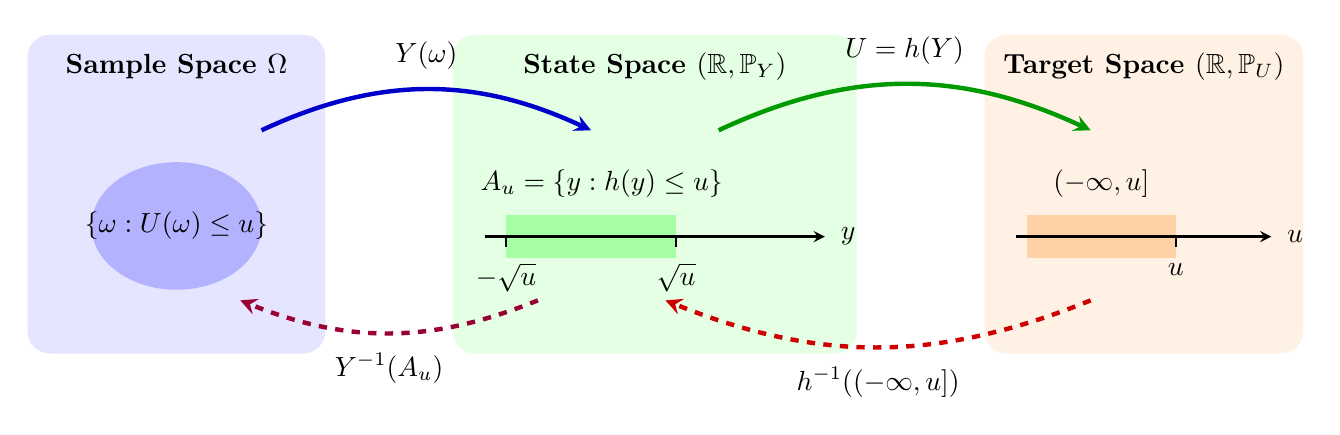
\begin{tikzpicture}[scale=1.35]
    % 1) Backgrounds / Shaded Regions
    \fill[blue!10, rounded corners=8pt] (-0.5, 0.2) rectangle (2.3, 3.2);
    \fill[green!10, rounded corners=8pt] (3.5, 0.2) rectangle (7.3, 3.2);
    \fill[orange!10, rounded corners=8pt] (8.5, 0.2) rectangle (11.5, 3.2);

    % Shaded sublevel sets inside spaces
    \fill[blue!30] (0.9, 1.4) ellipse (0.8 and 0.6);
    \fill[green!35] (4.0, 1.1) rectangle (5.6, 1.5);
    \fill[orange!35] (8.9, 1.1) rectangle (10.3, 1.5);

    % 2) Grid lines and Axes
    \draw[->, thick, >=stealth] (3.8, 1.3) -- (7.0, 1.3) node[right=2pt, black] {$y$};
    \draw[->, thick, >=stealth] (8.8, 1.3) -- (11.2, 1.3) node[right=2pt, black] {$u$};

    % Tick marks
    \draw[thick] (4.0, 1.3) -- (4.0, 1.2) node[below=2pt, black] {$-\sqrt{u}$};
    \draw[thick] (5.6, 1.3) -- (5.6, 1.2) node[below=2pt, black] {$\sqrt{u}$};
    \draw[thick] (10.3, 1.3) -- (10.3, 1.2) node[below=2pt, black] {$u$};

    % 3) Primary Plots (Mappings and Preimage Arrows)
    \draw[->, ultra thick, blue!80!black, >=stealth] (1.7, 2.3) to[bend left=25] node[above=3pt, black] {$\displaystyle Y(\omega)$} (4.8, 2.3);
    \draw[->, ultra thick, green!60!black, >=stealth] (6.0, 2.3) to[bend left=25] node[above=3pt, black] {$\displaystyle U = h(Y)$} (9.5, 2.3);
    \draw[->, ultra thick, red!80!black, dashed, >=stealth] (9.5, 0.7) to[bend left=22] node[below=3pt, black] {$\displaystyle h^{-1}((-\infty, u])$} (5.5, 0.7);
    \draw[->, ultra thick, purple!80!black, dashed, >=stealth] (4.3, 0.7) to[bend left=22] node[below=3pt, black] {$\displaystyle Y^{-1}(A_u)$} (1.5, 0.7);

    % 4) Labels and Text Nodes
    \node[black, font=\bfseries] at (0.9, 2.9) {Sample Space $\Omega$};
    \node[black] at (0.9, 1.4) {$\{\omega : U(\omega) \le u\}$};

    \node[black, font=\bfseries] at (5.4, 2.9) {State Space $(\R, \Prob_Y)$};
    \node[black] at (4.9, 1.8) {$A_u = \{y : h(y) \le u\}$};

    \node[black, font=\bfseries] at (10.0, 2.9) {Target Space $(\R, \Prob_U)$};
    \node[black] at (9.6, 1.8) {$(-\infty, u]$};
\end{tikzpicture}
\end{center}

\subsection{Heuristics and ``Cheats''}

\begin{enumerate}
    \item \textbf{The Boundary Continuity Sanity Check:} Because the integral of an integrable PDF over a single point or curve of Lebesgue measure zero is $0$, the derived CDF $F_U(u)$ of a continuous transformation of continuous random variables **must be continuous across all regime boundaries**. In Exercise 6.3, at the knot point $u = 6$, the left piece gives $\frac{(6+4)^2}{200} = \frac{100}{200} = \frac{1}{2}$ and the right piece gives $\frac{6-1}{10} = \frac{1}{2}$. In Exercise 6.6, at $u = 1$, both pieces equal $\frac{1}{2}$. If your piecewise CDF jumps at an interior boundary, your limits of integration are wrong!
    \item \textbf{The Leibniz Shortcut (Differentiating Before Evaluating):} If $F_U(u) = \int_{\alpha(u)}^{\beta(u)} f_Y(y)\,dy$, **do not** compute the antiderivative of $f_Y(y)$ if you only need the density $f_U(u)$! By the Leibniz Integral Rule:
    \[
        f_U(u) = \frac{d}{du} \int_{\alpha(u)}^{\beta(u)} f_Y(y)\,dy = f_Y(\beta(u))\beta'(u) - f_Y(\alpha(u))\alpha'(u).
    \]
    For instance, in Exercise 6.7 ($U = Z^2$), $F_U(u) = \int_{-\sqrt{u}}^{\sqrt{u}} \frac{1}{\sqrt{2\pi}}e^{-z^2/2}\,dz$ has no closed-form elementary antiderivative, yet differentiating the integral directly immediately yields $f_U(u)$.
    \item \textbf{Corner-Testing in Bivariate Domains:} To find the piecewise intervals of $u$ in a 2D problem $U = h(Y_1, Y_2)$, simply plug the coordinates $(y_1, y_2)$ of every **vertex (corner)** of the support region $S_{\mathbf{Y}}$ into $h(y_1, y_2)$. The resulting numbers are the exact transition thresholds for $u$.
\end{enumerate}

\subsection{Pitfalls and Fallacies}

\begin{itemize}
    \item \textbf{Pitfall 1: Differentiating Outside the Support.} Students frequently differentiate the algebraic formula for $F_U(u)$ without restricting $u$ to the image of the support $h(S_Y)$. Outside $h(S_Y)$, $F_U(u)$ is constant ($0$ or $1$), so its derivative is $0$. Always determine the minimum and maximum possible values of $U$ first.
    \item \textbf{Pitfall 2: Forgetting the Absolute Value / Sign Flip for Decreasing Transformations.} If $U = 1 - 2Y$, writing $F_U(u) = \Prob(1 - 2Y \le u) = \Prob\left(Y \le \frac{1-u}{2}\right)$ is a fatal algebraic error that produces a *negative* probability density function $f_U(u) < 0$.
    \item \textbf{Pitfall 3: Confusing $F^{-1}(u)$ with $1/F(u)$.} In the quantile inversion method, $F^{-1}(u)$ denotes the functional inverse (solving $F(y) = u$ for $y$), whereas in Exercise 6.19, $X = Y^{-1} = 1/Y$ denotes the algebraic reciprocal of the random variable.
    \item \textbf{Pitfall 4: Assuming $U = Y^2$ Always Doubles the Density.} As highlighted in our analysis of Exercise 6.1(c) vs. Exercise 6.2(c), the formula $f_U(u) = \frac{1}{2\sqrt{u}}[f_Y(\sqrt{u}) + f_Y(-\sqrt{u})]$ requires evaluating $f_Y(-\sqrt{u})$ according to the piecewise definition of $f_Y$. If $Y$ is only supported on $[0, 1]$, then $f_Y(-\sqrt{u}) = 0$, not $2(1 - (-\sqrt{u}))$!
\end{itemize}

\newpage
% ============================================================================
% PART 5: CONCEPTUAL SYNTHESIS AND THE "BIG PICTURE"
% ============================================================================
\section{Conceptual Synthesis and The ``Big Picture''}

\subsection{Thematic Connections}

The overarching theme of **The Method of Distribution Functions** is **Measure Transport via Set Preimages**. Across mathematics, whenever structure is transferred from a domain space $X$ to a codomain space $Y$ via a mapping $h : X \to Y$, forward mappings of points ($x \mapsto h(x)$) behave poorly if $h$ is non-injective or non-surjective, whereas inverse mappings of subsets ($B \mapsto h^{-1}(B)$) preserve all set-theoretic operations:
\[
    h^{-1}\left(\bigcup_{i} B_i\right) = \bigcup_{i} h^{-1}(B_i), \qquad h^{-1}\left(\bigcap_{i} B_i\right) = \bigcap_{i} h^{-1}(B_i), \qquad h^{-1}(B^c) = \big(h^{-1}(B)\big)^c.
\]
This exact set-theoretic isomorphism is why:
\begin{enumerate}
    \item In **Topology**, continuity is defined by preimages of open sets being open ($h^{-1}(V) \in \tau_X$).
    \item In **Measure Theory**, measurability is defined by preimages of Borel sets being measurable ($h^{-1}(B) \in \F$).
    \item In **Probability Theory**, the Method of Distribution Functions computes the pushforward law $\Prob_U$ by evaluating the base measure $\Prob_{\mathbf{Y}}$ on the preimage of half-rays: $F_U(u) = \Prob_{\mathbf{Y}}\big(h^{-1}((-\infty, u])\big)$.
\end{enumerate}

\subsection{Forward and Backward Links}

\begin{itemize}
    \item \textbf{Backward Links (Foundations Extended):}
    \begin{itemize}
        \item \textit{Univariate \& Bivariate Integration (Chapters 4 \& 5):} In Chapter 5, students computed static probabilities of fixed regions, such as $\Prob(Y_1 + Y_2 \le 1)$. Section 6.3 elevates that static upper limit to a dynamic parameter $u$, transforming a single numerical integral into a parameterized functional $F_U(u)$.
        \item \textit{Fundamental Theorem of Calculus:} Connects cumulative probability measure $F_U(u)$ back to local probability density $f_U(u) = F_U'(u)$.
    \end{itemize}
    \item \textbf{Forward Links (Bedrock for Advanced Topics):}
    \begin{itemize}
        \item \textit{The Method of Transformations / Jacobians (Section 6.4):} Applying the Chain Rule directly to $F_U(u) = F_Y(h^{-1}(u))$ (or $1 - F_Y(h^{-1}(u))$) immediately proves the univariate Jacobian formula $f_U(u) = f_Y(h^{-1}(u))\left|\frac{dh^{-1}(u)}{du}\right|$, which generalizes to the multivariable Jacobian determinant $|J|$.
        \item \textit{Order Statistics and Extreme Value Theory (Section 6.7):} To find the distribution of the maximum $Y_{(n)} = \max(Y_1, \dots, Y_n)$ or minimum $Y_{(1)} = \min(Y_1, \dots, Y_n)$ of i.i.d. random variables, Jacobian methods fail completely because $\max$ and $\min$ are not smooth bijections. The Method of Distribution Functions solves them effortlessly via set equivalence: $\{ \max_i Y_i \le u \} = \bigcap_{i=1}^n \{Y_i \le u\} \implies F_{Y_{(n)}}(u) = [F_Y(u)]^n$.
        \item \textit{Copula Theory (Sklar's Theorem) and Optimal Transport:} The Probability Integral Transform (Example 6.5, Exercises 6.15--6.18) proves that every continuous random variable $Y_i$ can be mapped to a uniform margin $U_i = F_{Y_i}(Y_i) \sim \text{Uniform}(0,1)$. In multivariate finance and machine learning, **Sklar's Theorem** states that any joint CDF $F(y_1, \dots, y_n)$ can be uniquely decomposed into its marginal CDFs and a **Copula** $C(F_1(y_1), \dots, F_n(y_n))$—a joint distribution function on $[0, 1]^n$ with uniform margins.
    \end{itemize}
\end{itemize}

\newpage
% ============================================================================
% PART 6: ABSTRACT REAL-WORLD MODELING (AI, ML, & QUANT FINANCE)
% ============================================================================
\section{Abstract Real-World Modeling (AI, ML, and Quant Finance)}

\subsection{Concrete Scenarios}

\begin{enumerate}
    \item \textbf{Generative Artificial Intelligence: Normalizing Flows and Diffusion Models.}
    Modern deep generative models (such as Normalizing Flows, Variational Autoencoders, and Score-Based Diffusion Models) aim to synthesize high-dimensional data $\mathbf{X} \in \R^d$ (e.g., images, molecular conformations, or audio waveforms) with an unknown complex density $p_{\mathbf{X}}(\mathbf{x})$. They achieve this by passing a simple base distribution $\mathbf{Z} \sim \mathcal{N}(\mathbf{0}, \mathbf{I}_d)$ or $\text{Uniform}(0,1)^d$ through a sequence of learnable, neural-network-parameterized pushforward transformations $\mathbf{X} = G_\theta(\mathbf{Z})$. In 1D autoregressive flows and Inverse Autoregressive Flows (IAF), each conditional distribution is explicitly modeled by learning a strictly monotonic cumulative distribution function $F_\theta(x_i \mid \mathbf{x}_{<i})$ and inverting it via the Method of Distribution Functions (Exercises 6.15--6.18).

    \item \textbf{Quantitative Finance: Credit Default Swaps (CDS) and Survival Time Simulation.}
    In structural and reduced-form credit risk models (e.g., Duffie-Singleton and Lando hazard-rate models), the default time $\tau$ of a corporate bond or sovereign entity is governed by a cumulative survival distribution $F_\tau(t) = \Prob(\tau \le t) = 1 - \exp\left(-\int_0^t \lambda(s)\,ds\right)$, where $\lambda(s)$ is the stochastic hazard rate (or default intensity). Notice that Exercise 6.15 ($F(y) = 1 - e^{-y^2}$, a Weibull/Rayleigh default law with linear hazard rate $\lambda(y) = 2y$) is an exact special case! Quantitative analysts price multi-name Collateralized Debt Obligations (CDOs) by simulating correlated uniform random variables $(U_1, \dots, U_n)$ from a Gaussian or Student-$t$ Copula and inverting each margin via $\tau_i = F_{\tau_i}^{-1}(U_i) = \Lambda_i^{-1}(-\ln(1 - U_i))$.

    \item \textbf{Algorithmic Trading and Market Microstructure: Queueing Delays at Limit Order Books.}
    High-frequency market makers place limit orders in electronic Limit Order Books (LOBs). As modeled in Exercises 6.10, 6.11, and 6.13, inter-arrival times of market orders and cancellations follow exponential or Weibull distributions. Determining the probability distribution of the total time-to-execution $U = \sum_{k=1}^q Y_k$ (Exercise 6.13) or the net sojourn time at the top of the book $U = Y_1 - Y_2$ (Exercise 6.10) via the Method of Distribution Functions allows execution algorithms to compute optimal order-placement depths and fill probabilities.
\end{enumerate}

\subsection{Model Problem Setup: Quantitative Research Framework for Derivative Pricing and Risk-Neutral Density Extraction}

We now formulate a rigorous mathematical model bridging **Stochastic Calculus**, **Derivative Pricing**, and **The Method of Distribution Functions**.

\subsubsection*{1. Filtered Probability Space and Stochastic Dynamics}
Let $(\Omega, \F, \{\F_t\}_{t \in [0, T]}, \Q)$ be a complete filtered probability space equipped with the **risk-neutral martingale measure** $\Q$, supporting a standard $1$-dimensional Brownian motion $\{W_t\}_{t \in [0, T]}$. Suppose the underlying asset price $S_t$ follows Geometric Brownian Motion (GBM) under $\Q$ with constant risk-free rate $r \in \R$ and volatility $\sigma > 0$:
\[
    dS_t = r S_t\,dt + \sigma S_t\,dW_t, \qquad S_0 > 0.
\]
By **It\^{o}'s Lemma** applied to the logarithmic transformation $Y_t = \ln S_t$:
\[
    d(\ln S_t) = \left(r - \frac{1}{2}\sigma^2\right)dt + \sigma\,dW_t \implies S_T = S_0 \exp\left( \left(r - \frac{1}{2}\sigma^2\right)T + \sigma W_T \right).
\]
Since $W_T \sim \mathcal{N}(0, T)$, we can write $W_T = \sqrt{T} Z$ where $Z \sim \mathcal{N}(0, 1)$.

\subsubsection*{2. Deriving the Terminal Asset Density and Quadratic Variance Swaps via Distribution Functions}
Define the standardized log-return $Y = \left(r - \frac{1}{2}\sigma^2\right)T + \sigma\sqrt{T}Z \sim \mathcal{N}(\mu_T, \sigma_T^2)$, where $\mu_T = \left(r - \frac{1}{2}\sigma^2\right)T$ and $\sigma_T = \sigma\sqrt{T}$.
\begin{enumerate}
    \item \textbf{Terminal Spot Price Distribution ($S_T = S_0 e^Y$):} Using the Method of Distribution Functions for $s > 0$:
    \[
        F_{S_T}(s) = \Q(S_0 e^Y \le s) = \Q\left(Y \le \ln\left(\frac{s}{S_0}\right)\right) = \Phi\left( \frac{\ln(s/S_0) - \mu_T}{\sigma_T} \right),
    \]
    where $\Phi(z) = \int_{-\infty}^z \frac{1}{\sqrt{2\pi}}e^{-t^2/2}\,dt$. Differentiating with respect to $s$ yields the **Log-Normal Risk-Neutral Density**:
    \[
        f_{S_T}(s) = \frac{dF_{S_T}(s)}{ds} = \frac{1}{s\sigma\sqrt{2\pi T}} \exp\left( -\frac{\big(\ln(s/S_0) - (r - \frac{1}{2}\sigma^2)T\big)^2}{2\sigma^2 T} \right), \quad s > 0.
    \]
    \item \textbf{Realized Single-Period Variance Payoff ($U = Z^2$):} A discrete variance contract pays proportional to the squared standardized shock $U = Z^2$. By Exercise 6.7, the Method of Distribution Functions establishes that $U \sim \chi^2_1 = \text{Gamma}\left(\frac{1}{2}, 2\right)$ with density $f_U(u) = \frac{1}{\sqrt{2\pi}}u^{-1/2}e^{-u/2}\mathbf{1}_{(0,\infty)}(u)$.
\end{enumerate}

\subsubsection*{3. Breeden-Litzenberger Theorem and Inverse Transform Calibration}
Suppose the true market distribution $F_{S_T}(K) = \Q(S_T \le K)$ deviates from log-normality (exhibiting volatility smiles and heavy Pareto tails as in Exercise 6.18). Let $C(K, T)$ denote the observable market price of a European call option with strike $K > 0$ and maturity $T$:
\[
    C(K, T) = e^{-rT} \E^{\Q}\big[(S_T - K)^+\big] = e^{-rT} \int_{K}^{\infty} (s - K) f_{S_T}(s)\,ds.
\]
Applying the **Leibniz Integral Rule** twice with respect to the strike threshold $K$ (the exact dual of the Method of Distribution Functions):
\begin{align*}
    \frac{\partial C(K, T)}{\partial K} &= e^{-rT} \left[ -(K - K)f_{S_T}(K) + \int_{K}^{\infty} (-1) f_{S_T}(s)\,ds \right] = -e^{-rT}\big(1 - F_{S_T}(K)\big), \\
    \frac{\partial^2 C(K, T)}{\partial K^2} &= e^{-rT} \frac{dF_{S_T}(K)}{dK} = e^{-rT} f_{S_T}(K).
\end{align*}
This yields the celebrated **Breeden-Litzenberger Formulas**:
\[
    F_{S_T}(K) = 1 + e^{rT} \frac{\partial C(K, T)}{\partial K}, \qquad f_{S_T}(K) = e^{rT} \frac{\partial^2 C(K, T)}{\partial K^2}.
\]
Once $F_{S_T}(K)$ is extracted non-parametrically from market option prices, a Monte Carlo engine generates exact risk-neutral asset trajectories by drawing $U \sim \text{Uniform}(0, 1)$ and applying the quantile inversion of Section 6.3:
\[
    \widehat{S}_T = F_{S_T}^{-1}(U) = \inf\left\{ K > 0 : 1 + e^{rT}\frac{\partial C(K, T)}{\partial K} \ge U \right\}.
\]

\newpage
% ============================================================================
% PART 7: COMMON VARIATIONS AND UNTESTED CONCEPTS
% ============================================================================
\section{Common Variations and Untested Concepts}

While the assigned exercises thoroughly test affine, quadratic, bivariate additive, bivariate multiplicative, and quantile-inversion problems, standard advanced university examinations frequently test three critical variations omitted from the homework set:

\subsection{Variation 1: Mixed Discrete-Continuous (Censored / ReLU) Transformations}

In deep learning (the **Rectified Linear Unit**, $\text{ReLU}(y) = \max(0, y)$) and insurance deductibles (where claims below $d$ pay $0$), a continuous random variable $Y$ is passed through a transformation that collapses an entire interval of positive probability onto a single point mass.

\begin{example}[Distribution of a ReLU-Transformed Random Variable]
Let $Y \sim \mathcal{N}(0, 1)$ and define $U = \max(0, Y)$. Find the cumulative distribution function $F_U(u)$ and explain why $U$ does not possess a classical probability density function on $\R$.
\end{example}

\textbf{Rigorous Solution:}
\begin{itemize}
    \item \textit{Case 1 ($u < 0$):} Since $U = \max(0, Y) \ge 0$ for all $\omega \in \Omega$, the event $\{U \le u\} = \emptyset$. Thus $F_U(u) = 0$.
    \item \textit{Case 2 ($u = 0$):} Since $\max(0, Y) \le 0 \iff Y \le 0$, we have:
    \[
        F_U(0) = \Prob(U \le 0) = \Prob(Y \le 0) = \Phi(0) = \frac{1}{2}.
    \]
    Notice that $\lim_{u \to 0^-} F_U(u) = 0 \neq \frac{1}{2} = F_U(0)$! Therefore, $F_U(u)$ has a jump discontinuity of size $\Delta F_U(0) = \Prob(U = 0) = \frac{1}{2}$ at $u = 0$.
    \item \textit{Case 3 ($u > 0$):} For $u > 0$, $\max(0, Y) \le u \iff Y \le u$. Thus $F_U(u) = \Prob(Y \le u) = \Phi(u)$.
\end{itemize}
Summarizing:
\[
    F_U(u) = \begin{cases} 0, & u < 0, \\ \Phi(u), & u \ge 0. \end{cases}
\]
By the **Lebesgue Decomposition Theorem**, the pushforward measure $\Prob_U = \frac{1}{2}\delta_0 + \Prob_{U,\text{ac}}$ is a mixture of a **Dirac point mass** $\delta_0$ at $u = 0$ (singular with respect to Lebesgue measure) and an absolutely continuous component with density $\frac{1}{\sqrt{2\pi}}e^{-u^2/2}\mathbf{1}_{(0,\infty)}(u)$. Using generalized functions (Schwartz distributions), its generalized density is written as $f_U(u) = \frac{1}{2}\delta(u) + \frac{1}{\sqrt{2\pi}}e^{-u^2/2}\mathbf{1}_{(0,\infty)}(u)$. \hfill $\blacksquare$

\subsection{Variation 2: Quotient of Independent Random Variables (The Cauchy Ratio)}

The homework tests sums ($Y_1 + Y_2$), differences ($Y_1 - Y_2$), and products ($Y_1 Y_2$), but omits **quotients** $U = Y_1 / Y_2$.

\begin{example}[Ratio of Independent Exponential Random Variables]
Let $Y_1, Y_2 \stackrel{\text{i.i.d.}}{\sim} \text{Exponential}(1)$. Use the Method of Distribution Functions to find the PDF of $U = \dfrac{Y_1}{Y_2}$.
\end{example}

\textbf{Rigorous Solution:}
Since $Y_1, Y_2 > 0$ almost surely with joint density $f(y_1, y_2) = e^{-(y_1 + y_2)}$ on $(0, \infty)^2$, we have $U > 0$, so $F_U(u) = 0$ for $u \le 0$. For $u > 0$, the event $\left\{\frac{Y_1}{Y_2} \le u\right\} = \{Y_1 \le u Y_2\}$ is the sector in the first quadrant bounded by $y_1 = 0$ and the ray $y_1 = u y_2$:
\begin{align*}
    F_U(u) &= \Prob\left(\frac{Y_1}{Y_2} \le u\right) = \int_{0}^{\infty} \int_{0}^{u y_2} e^{-y_1} e^{-y_2}\,dy_1\,dy_2 = \int_{0}^{\infty} e^{-y_2}\left(1 - e^{-u y_2}\right) dy_2 \\
    &= \int_{0}^{\infty} e^{-y_2}\,dy_2 - \int_{0}^{\infty} e^{-(1 + u)y_2}\,dy_2 = 1 - \frac{1}{1 + u} = \frac{u}{1 + u}, \quad u > 0.
\end{align*}
Differentiating with respect to $u$ yields the heavy-tailed ** Lomax / $F(2,2)$** density (which possesses no finite mean!):
\[
    f_U(u) = \frac{dF_U(u)}{du} = \begin{cases} \dfrac{1}{(1 + u)^2}, & u > 0, \\[6pt] 0, & \text{elsewhere.} \end{cases} \quad \blacksquare
\]

\subsection{Variation 3: Asymmetric Folding (Piecewise 1-to-1 and 2-to-1 Regimes)}

When $Y$ is supported on an asymmetric interval $[a, b]$ containing $0$ (such as $[-1, 2]$) and $U = Y^2$, the transformation $y \mapsto y^2$ is **two-to-one** on $[-1, 1]$ ($0 < u \le 1$) but **one-to-one** on $(1, 2]$ ($1 < u \le 4$).

\begin{example}[Asymmetric Quadratic Folding]
Let $Y \sim \text{Uniform}(-1, 2)$, so $f_Y(y) = \frac{1}{3}$ on $[-1, 2]$. Find the PDF of $U = Y^2$.
\end{example}

\textbf{Rigorous Solution:}
Since $Y \in [-1, 2]$, $U = Y^2 \in [0, 4]$.
\begin{itemize}
    \item \textit{Regime 1 ($0 < u \le 1$):} Both $-\sqrt{u}$ and $\sqrt{u}$ lie inside $[-1, 2]$. Thus:
    \[
        F_U(u) = \Prob(-\sqrt{u} \le Y \le \sqrt{u}) = \int_{-\sqrt{u}}^{\sqrt{u}} \frac{1}{3}\,dy = \frac{2\sqrt{u}}{3} \implies f_U(u) = \frac{1}{3\sqrt{u}}.
    \]
    \item \textit{Regime 2 ($1 < u \le 4$):} Here $-\sqrt{u} < -1$, so intersecting $[-\sqrt{u}, \sqrt{u}]$ with $[-1, 2]$ gives $[-1, \sqrt{u}]$:
    \[
        F_U(u) = \Prob(-1 \le Y \le \sqrt{u}) = \int_{-1}^{\sqrt{u}} \frac{1}{3}\,dy = \frac{\sqrt{u} + 1}{3} \implies f_U(u) = \frac{1}{6\sqrt{u}}.
    \]
\end{itemize}
Thus,
\[
    f_U(u) = \begin{cases} \dfrac{1}{3\sqrt{u}}, & 0 < u \le 1, \\[6pt] \dfrac{1}{6\sqrt{u}}, & 1 < u \le 4, \\[6pt] 0, & \text{elsewhere.} \end{cases} \quad \blacksquare
\]

\newpage
% ============================================================================
% PART 8: ADVANCED DIAGNOSTIC TESTING: "FIND THE FLAW"
% ============================================================================
\section{Advanced Diagnostic Testing: ``Find the Flaw''}

Below are five advanced problems accompanied by seemingly rigorous step-by-step proofs. Each proof contains **one subtle, fatal mathematical or logical flaw**. Act as the examiner: locate the exact line where the proof breaks down, explain the theoretical violation, and construct the corrected derivation before consulting the Solution Key.

\subsection{Diagnostic Problems and Flawed Proofs}

\subsubsection*{Problem 1: The Vanishing Support Phantom}
\textbf{Statement:} Let $Y$ have PDF $f_Y(y) = 2y$ for $0 \le y \le 1$, and $0$ elsewhere. Find the PDF of $U = Y^2$.

\textbf{Flawed Solution:}
\begin{enumerate}[label=Step \arabic*:]
    \item For $u \le 0$, $F_U(u) = \Prob(Y^2 \le u) = 0$.
    \item For $0 < u \le 1$, we use the general quadratic distribution formula derived in Section 6.3 (page 305 of the text):
    \[
        F_U(u) = \Prob(-\sqrt{u} \le Y \le \sqrt{u}) = F_Y(\sqrt{u}) - F_Y(-\sqrt{u}).
    \]
    \item Differentiating with respect to $u$ yields:
    \[
        f_U(u) = \frac{1}{2\sqrt{u}}\Big[ f_Y(\sqrt{u}) + f_Y(-\sqrt{u}) \Big].
    \]
    \item Substituting $f_Y(y) = 2y$ into the formula gives:
    \[
        f_U(u) = \frac{1}{2\sqrt{u}}\Big[ 2(\sqrt{u}) + 2(-\sqrt{u}) \Big] = \frac{1}{2\sqrt{u}}(0) = 0, \quad 0 < u \le 1.
    \]
\end{enumerate}

\hrulefill

\subsubsection*{Problem 2: The Decreasing Transformation Trap}
\textbf{Statement:} Let $Y \sim \text{Exponential}(1)$ with PDF $f_Y(y) = e^{-y}$ for $y \ge 0$. Find the PDF of $U = e^{-Y}$.

\textbf{Flawed Solution:}
\begin{enumerate}[label=Step \arabic*:]
    \item Since $Y \ge 0$, as $y$ ranges from $0$ to $\infty$, $u = e^{-y}$ ranges over $(0, 1]$. Thus $F_U(u) = 0$ for $u \le 0$ and $F_U(u) = 1$ for $u > 1$.
    \item For $0 < u \le 1$, we apply the Method of Distribution Functions by taking natural logarithms:
    \[
        F_U(u) = \Prob(e^{-Y} \le u) = \Prob(-Y \le \ln u) = \Prob(Y \le -\ln u).
    \]
    \item Since $-\ln u \ge 0$ for $0 < u \le 1$, substituting into the Exponential CDF $F_Y(y) = 1 - e^{-y}$ gives:
    \[
        F_U(u) = 1 - e^{-(-\ln u)} = 1 - u.
    \]
    \item Differentiating with respect to $u$ gives $f_U(u) = \frac{d}{du}(1 - u) = -1$, and taking the absolute value of the Jacobian gives $f_U(u) = 1$ for $0 < u \le 1$.
\end{enumerate}

\hrulefill

\subsubsection*{Problem 3: The Bivariate Boundary Mirage}
\textbf{Statement:} Let $(Y_1, Y_2)$ have joint PDF $f(y_1, y_2) = 1$ on the rectangle $0 \le y_1 \le 2$, $0 \le y_2 \le 1$, and $0$ elsewhere. Find $F_U(u)$ for $U = Y_1 + Y_2$ when $1 < u \le 2$.

\textbf{Flawed Solution:}
\begin{enumerate}[label=Step \arabic*:]
    \item The minimum of $U$ on $[0, 2] \times [0, 1]$ is $0$ and the maximum is $2 + 1 = 3$.
    \item For any $u \in (1, 2]$, the event $\{U \le u\} = \{Y_1 + Y_2 \le u\}$ lies below the line $y_1 + y_2 = u$ in the first quadrant.
    \item Integrating $f(y_1, y_2) = 1$ over the triangle bounded by $y_1 = 0$, $y_2 = 0$, and $y_1 + y_2 = u$:
    \[
        F_U(u) = \int_{0}^{u} \int_{0}^{u - y_1} 1\,dy_2\,dy_1 = \int_{0}^{u} (u - y_1)\,dy_1 = \frac{u^2}{2}, \quad 1 < u \le 2.
    \]
\end{enumerate}

\hrulefill

\subsubsection*{Problem 4: The Non-Monotone Quantile Inversion Fallacy}
\textbf{Statement:} Let $Y$ have CDF $F_Y(y) = \frac{y^3 + 1}{2}$ for $-1 \le y \le 1$ (from Exercise 6.2). Suppose a student wants to simulate $W = Y^2$ from $U \sim \text{Uniform}(0, 1)$.

\textbf{Flawed Solution:}
\begin{enumerate}[label=Step \arabic*:]
    \item By the Quantile Inversion Theorem, $Y = F_Y^{-1}(U) = (2U - 1)^{1/3}$ has CDF $F_Y(y)$.
    \item Since $W = h(Y) = Y^2$ and $F_W(w) = F_Y(\sqrt{w})$ on $[0, 1]$, we solve $F_Y(\sqrt{w}) = u$:
    \[
        \frac{w^{3/2} + 1}{2} = u \implies w = (2u - 1)^{2/3}.
    \]
    \item Therefore, the CDF of $W = Y^2$ is $F_W(w) = \frac{w^{3/2} + 1}{2}$ for $0 \le w \le 1$, and $f_W(w) = \frac{3}{4}\sqrt{w}$.
\end{enumerate}

\hrulefill

\subsubsection*{Problem 5: The Dependent Convolution Trap}
\textbf{Statement:} Let $(Y_1, Y_2)$ have uniform joint density $f(y_1, y_2) = 2$ on the simplex $0 \le y_1 \le 1, 0 \le y_2 \le 1, y_1 + y_2 \le 1$ (as in Exercise 6.9). Find the PDF of $U = Y_1 + Y_2$.

\textbf{Flawed Solution:}
\begin{enumerate}[label=Step \arabic*:]
    \item From Exercise 6.9(c), the marginal densities of $Y_1$ and $Y_2$ are $f_1(y_1) = 2(1 - y_1)\mathbf{1}_{[0,1]}(y_1)$ and $f_2(y_2) = 2(1 - y_2)\mathbf{1}_{[0,1]}(y_2)$.
    \item For $0 \le u \le 1$, the CDF of $U = Y_1 + Y_2$ is obtained by integrating the product of the marginals over $y_1 + y_2 \le u$:
    \[
        F_U(u) = \int_{0}^{u} \int_{0}^{u - y_1} f_1(y_1)f_2(y_2)\,dy_2\,dy_1 = \int_{0}^{u} \int_{0}^{u - y_1} 4(1 - y_1)(1 - y_2)\,dy_2\,dy_1.
    \]
    \item Differentiating with respect to $u$ gives $f_U(u) = \int_0^u 4(1 - y_1)(1 - u + y_1)\,dy_1 = 4u - 4u^2 + \frac{2}{3}u^3$.
\end{enumerate}

\newpage
\subsection{Solution Key and True Resolutions}

\begin{enumerate}
    \item \textbf{Resolution to Problem 1 (The Vanishing Support Phantom):}
    \begin{itemize}
        \item \textit{The Flaw:} **Step 4** violates the piecewise definition of $f_Y(y)$. Because $f_Y(y) = 0$ for all $y < 0$, evaluating $f_Y$ at $-\sqrt{u} < 0$ yields $f_Y(-\sqrt{u}) = 0$, **not** $2(-\sqrt{u})$!
        \item \textit{Correct Step:} Substituting $f_Y(\sqrt{u}) = 2\sqrt{u}$ and $f_Y(-\sqrt{u}) = 0$ into Step 3 gives:
        \[
            f_U(u) = \frac{1}{2\sqrt{u}}\big[ 2\sqrt{u} + 0 \big] = 1, \quad 0 < u \le 1,
        \]
        so $U = Y^2 \sim \text{Uniform}(0, 1)$ (which also follows immediately from the Probability Integral Transform since $F_Y(y) = y^2$!).
    \end{itemize}

    \item \textbf{Resolution to Problem 2 (The Decreasing Transformation Trap):}
    \begin{itemize}
        \item \textit{The Flaw:} **Step 2** fails to reverse the inequality sign when multiplying $-Y \le \ln u$ by $-1$. Furthermore, in Step 4, a cumulative distribution function $F_U(u)$ can **never** have a negative derivative $F_U'(u) = -1 < 0$; taking an arbitrary absolute value at the end masks the algebraic error in $F_U(u)$.
        \item \textit{Correct Step:} In Step 2, $-Y \le \ln u \iff Y \ge -\ln u$. Therefore:
        \[
            F_U(u) = \Prob(Y \ge -\ln u) = 1 - F_Y(-\ln u) = 1 - \left(1 - e^{-(-\ln u)}\right) = u, \quad 0 < u \le 1.
        \]
        Differentiating $F_U(u) = u$ directly gives $f_U(u) = 1$ on $(0, 1]$ without any artificial sign correction.
    \end{itemize}

    \item \textbf{Resolution to Problem 3 (The Bivariate Boundary Mirage):}
    \begin{itemize}
        \item \textit{The Flaw:} **Step 3** integrates over the region $0 \le y_2 \le u - y_1$ for $0 \le y_1 \le u$. However, when $1 < u \le 2$ and $y_1 < u - 1$, the upper limit $y_2 = u - y_1$ exceeds $1$, exiting the top boundary $y_2 = 1$ of the support rectangle $[0, 2] \times [0, 1]$ where $f(y_1, y_2) = 0$!
        \item \textit{Correct Step:} For $1 < u \le 2$, we must split the $y_1$ integral at $y_1 = u - 1$ (where $u - y_1 = 1$), or integrate with respect to $y_1$ first from $0$ to $u - y_2$ as $y_2$ ranges from $0$ to $1$:
        \[
            F_U(u) = \int_{0}^{1} \int_{0}^{u - y_2} 1\,dy_1\,dy_2 = \int_{0}^{1} (u - y_2)\,dy_2 = u - \frac{1}{2}, \quad 1 < u \le 2.
        \]
    \end{itemize}

    \item \textbf{Resolution to Problem 4 (The Non-Monotone Quantile Inversion Fallacy):}
    \begin{itemize}
        \item \textit{The Flaw:} **Step 2** asserts that $F_W(w) = F_Y(\sqrt{w})$ on $[0, 1]$. Because $Y$ takes negative values on $[-1, 0)$, the event $\{Y^2 \le w\}$ is $\{-\sqrt{w} \le Y \le \sqrt{w}\}$, so $F_W(w) = F_Y(\sqrt{w}) - F_Y(-\sqrt{w})$, not $F_Y(\sqrt{w})$! Notice that the flawed $F_W(0) = \frac{1}{2} \neq 0$.
        \item \textit{Correct Step:} As shown in Exercise 6.2(c), $F_W(w) = \frac{w^{3/2} + 1}{2} - \frac{(-w^{3/2}) + 1}{2} = w^{3/2}$ for $0 \le w \le 1$, so $f_W(w) = \frac{3}{2}\sqrt{w}$ and the quantile transform is $W = U^{2/3}$.
    \end{itemize}

    \item \textbf{Resolution to Problem 5 (The Dependent Convolution Trap):}
    \begin{itemize}
        \item \textit{The Flaw:} **Step 2** replaces the true joint density $f(y_1, y_2) = 2$ with the product of the marginal densities $f_1(y_1)f_2(y_2) = 4(1-y_1)(1-y_2)$. Random variables $Y_1$ and $Y_2$ supported on a triangular simplex $y_1 + y_2 \le 1$ are **strictly dependent** ($f(y_1, y_2) \neq f_1(y_1)f_2(y_2)$)!
        \item \textit{Correct Step:} One must integrate the actual joint density $f(y_1, y_2) = 2$ over $\{y_1 \ge 0, y_2 \ge 0 : y_1 + y_2 \le u\}$, yielding $F_U(u) = u^2$ and $f_U(u) = 2u$ for $0 \le u \le 1$, as proven in Exercise 6.9(a).
    \end{itemize}
\end{enumerate}

\end{document}